%% abtex2-modelo-trabalho-academico.tex, v-1.9.6 laurocesar
%% Copyright 2012-2016 by abnTeX2 group at http://www.abntex.net.br/
%%
%% This work may be distributed and/or modified under the
%% conditions of the LaTeX Project Public License, either version 1.3
%% of this license or (at your option) any later version.
%% The latest version of this license is in
%%   http://www.latex-project.org/lppl.txt
%% and version 1.3 or later is part of all distributions of LaTeX
%% version 2005/12/01 or later.
%%
%% This work has the LPPL maintenance status `maintained'.
%%
%% The Current Maintainer of this work is the abnTeX2 team, led
%% by Lauro César Araujo. Further information are available on
%% http://www.abntex.net.br/
%%
%% This work consists of the files abntex2-modelo-trabalho-academico.tex,
%% abntex2-modelo-include-comandos and abntex2-modelo-references.bib
%%

% ------------------------------------------------------------------------
% ------------------------------------------------------------------------
% abnTeX2: Modelo de Trabalho Academico (tese de doutorado, dissertacao de
% mestrado e trabalhos monograficos em geral) em conformidade com
% ABNT NBR 14724:2011: Informacao e documentacao - Trabalhos academicos -
% Apresentacao
% ------------------------------------------------------------------------
% ------------------------------------------------------------------------

\documentclass[
	% -- opções da classe memoir --
	12pt,				% tamanho da fonte
%	openright,			% capítulos começam em pág ímpar (insere página vazia caso preciso)
	oneside,			% para impressão em recto e verso. Oposto a oneside
%    oneside,			% Oposto a twoside
	a4paper,			% tamanho do papel.
	% -- opções da classe abntex2 --
	%chapter=TITLE,		% títulos de capítulos convertidos em letras maiúsculas
	%section=TITLE,		% títulos de seções convertidos em letras maiúsculas
	%subsection=TITLE,	% títulos de subseções convertidos em letras maiúsculas
	%subsubsection=TITLE,% títulos de subsubseções convertidos em letras maiúsculas
	% -- opções do pacote babel --
	english,			% idioma adicional para hifenização
	french,				% idioma adicional para hifenização
	spanish,			% idioma adicional para hifenização
	brazil				% o último idioma é o principal do documento
	]{abntex2}

% ---
% Pacotes 
% ---
\usepackage{lmodern}			% Usa a fonte Latin Modern			
\usepackage[T1]{fontenc}		% Selecao de codigos de fonte.
\usepackage[utf8]{inputenc}		% Codificacao do documento (conversão automática dos acentos)
\usepackage{lastpage}			% Usado pela Ficha catalográfica
\usepackage{indentfirst}		% Indenta o primeiro parágrafo de cada seção.
\usepackage{color}				% Controle das cores
\usepackage{graphicx}			% Inclusão de gráficos
\usepackage{microtype} 			% para melhorias de justificação

\usepackage{lipsum}				% para geração de dummy text

\usepackage[brazilian,hyperpageref]{backref}	 % Paginas com as citações na bibl
\usepackage[alf]{abntex2cite}	% Citações padrão ABNT
\usepackage{float}
% ---
% CONFIGURAÇÕES DE PACOTES
% ---

% ---
% Configurações do pacote backref
% Usado sem a opção hyperpageref de backref
\renewcommand{\backrefpagesname}{Citado na(s) página(s):~}
% Texto padrão antes do número das páginas
\renewcommand{\backref}{}
% Define os textos da citação
\renewcommand*{\backrefalt}[4]{
	\ifcase #1 %
		Nenhuma citação no texto.%
	\or
		Citado na página #2.%
	\else
		Citado #1 vezes nas páginas #2.%
	\fi}%
% ---

% ---
% Informações de dados para CAPA e FOLHA DE ROSTO
% ---
\titulo{Conversor tensão-frequência CMOS de baixo consumo e baixa potência para aplicação em redes de sensores sem fio}
\autor{Danilo Lopes Barbosa}
\local{Brasil}
\data{Novembro de 2020}
\orientador{Robson Luiz Moreno}
\instituicao{%
  Universidade Federal de Itajubá -- UNIFEI
  \par
  Instituto de Engenharia de Sistemas e Tecnologia da Informação
  \par
  Engenharia da Computação}
\tipotrabalho{Trabalho Final de Graduação}
% O preambulo deve conter o tipo do trabalho, o objetivo,
% o nome da instituição e a área de concentração
\preambulo{Monografia referente ao Trabalho Final de Graduação do curso de Engenharia da Computação da Universidade Federal de Itajubá}
% ---


% ---
% Configurações de aparência do PDF final

% alterando o aspecto da cor azul
\definecolor{blue}{RGB}{41,5,195}

% informações do PDF
\makeatletter
\hypersetup{
     	%pagebackref=true,
		pdftitle={\@title},
		pdfauthor={\@author},
    	pdfsubject={\imprimirpreambulo},
	    pdfcreator={LaTeX with abnTeX2},
		pdfkeywords={abnt}{latex}{abntex}{abntex2}{trabalho acadêmico},
		colorlinks=true,       		% false: boxed links; true: colored links
    	linkcolor=blue,          	% color of internal links
    	citecolor=blue,        		% color of links to bibliography
    	filecolor=magenta,      		% color of file links
		urlcolor=blue,
		bookmarksdepth=4
}
\makeatother
% ---

% ---
% Espaçamentos entre linhas e parágrafos
% ---

% O tamanho do parágrafo é dado por:
\setlength{\parindent}{1.3cm}

% Controle do espaçamento entre um parágrafo e outro:
\setlength{\parskip}{0.2cm}  % tente também \onelineskip

% ---
% compila o indice
% ---
\makeindex
% ---

% ----
% Início do documento
% ----
\begin{document}

% Seleciona o idioma do documento (conforme pacotes do babel)
%\selectlanguage{english}
\selectlanguage{brazil}

% Retira espaço extra obsoleto entre as frases.
\frenchspacing

% ----------------------------------------------------------
% ELEMENTOS PRÉ-TEXTUAIS
% ----------------------------------------------------------
% Capa e Folha de Rosto
\imprimircapa
\imprimirfolhaderosto*
% ---

% ---
% Dedicatória
% ---
\begin{dedicatoria}
   \vspace*{\fill}
   \centering
   \noindent
   \textit{ Aos meus pais e professores.} \vspace*{\fill}
\end{dedicatoria}
% ---

% ---
% Agradecimentos
% ---
\begin{agradecimentos}
Agradeço a meus professores da UNIFEI, em especial meu orientador Robson, pelo conhecimento sem o qual a realização desse trabalho não seria possível. Agradeço também aos professores Behzad Razavi e Ali Hajimiri cujos cursos sobre eletrônica analógica, generosamente disponibilizados de forma gratuita na internet, foram essenciais como complementação para as disciplinas que cursei ao longo do curso de Engenharia da Computação. 
\end{agradecimentos}
% ---

% ---
% Epígrafe
% ---
\begin{epigrafe}
    \vspace*{\fill}
	\begin{flushright}
		\textit{"Pensar, analizar, inventar [...] son la normal
		respiración de la inteligencia. Glorificar el ocasional cumplimiento de esa función [...] es confesar nuestra languidez o nuestra barbarie. Todo hombre debe ser capaz de todas las ideas y entiendo do que en el porvenir lo será"}
		\\
		\textbf{Jorge Luis Borges}
	\end{flushright}
\end{epigrafe}
% ---

% ---
% RESUMOS
% ---

% resumo em português
\setlength{\absparsep}{18pt} % ajusta o espaçamento dos parágrafos do resumo
\begin{resumo}
O uso de métodos de conversão \textit{quasi} digitais como alternativas de baixo custo a conversores analógico-digitais convencionais (ADCs), em aplicações portáteis, tem sido cada vez mais popular ao longo das últimas décadas. Tendo como motivação possíveis aplicações em redes de sensores sem fio (WSNs), o presente trabalho se propôs ao projeto de um conversor tensão-frequência (VFC) de baixo consumo e baixa potência. Uma breve revisão bibliográfica foi realizada a respeito do assunto, seguida do projeto de um VFC multivibrador composto por 3 blocos: um conversor V-I com entrada \textit{rail-to-rail} implementado com \textit{feedforward voltage attenuation} (FFVA), um integrador bidirecional de baixo consumo e um \textit{voltage window comparator} atuando como circuito de controle. O circuito foi projetado com auxílio do software Cadence Virtuoso, utilizando tecnologia CMOS IBM 130nm, tensão de alimentação de 1,2V e uma corrente de polarização de 5$\mu$A. Para análise de desempenho, simulações foram realizadas com o simulador Spectre. O VFC projetado apresentou consumo de 424 $\mu$W, faixa de entrada de [0 - 1,1 V], faixa de saída de [7,44 kHz - 606,1 kHz] e erro de linearidade de 0,49\%. O OTA projetado como entrada para o circuito apresentou faixa de entrada \textit{rail-to-rail} com uma variação máxima de transcondutância de 5,08\%. Os resultados obtidos foram satisfatórios para o escopo do projeto, principalmente os obtidos pelo conversor V-I projetado, com as frequências de saída estando na faixa adequada para a especificação e o consumo de potência mostrando-se razoável. O erro de linearidade obtido foi baixo o suficiente, porém ainda pode ser considerado alto quando comparado a outros trabalhos similares. Por isso, fica como sugestão para trabalhos futuros a implementação de métodos para otimização da linearidade e consumo do VFC, bem como a implementação de compensação de temperatura para o circuito.       

 \textbf{Palavras-chave}: CMOS. VFC. Microeletrônica. 
\end{resumo}

% resumo em inglês
\begin{resumo}[Abstract]
 \begin{otherlanguage*}{english}
The use of quasi-digital conversion methods as low cost alternatives to conventional analog to digital converters (ADC), on portable applications, has become increasingly popular over the last decades. Using possible applications on wireless sensor networks (WSNs) as motivation, the design of a  low voltage, low power voltage to frequency converter (VFC) was proposed in this work. A brief literature review was made on the subject, followed by the design of a multivibrator VFC made of 3 blocks: A rail-to-rail input V-I converter implemented by feedforward voltage attenuation (FFVA), a low power bidirectional current integrator and a voltage window comparator as a control circuit. The circuit was designed on Cadence Virtuoso software, using IBM 130nm CMOS technology, supply voltage of 1.2V and a bias current of 5 $\mu$A. The Spectre simulator was used for simulations and performance analysis. The designed VFC presented 424 $\mu$W of power consumption, input voltage range of [0 - 1,1 V], output frequency range of [7,44 kHz - 606,1 kHz] and a 0,49\% linearity error. The designed input OTA showed rail-to-rail input range and a maximum total input transconductance deviation of 5,08\%. These where satisfactory results given the scope of the project, especially the ones obtained by the V-I converter, with the output frequencies being on an adequate range according to the specification and the power consumption being reasonably low. The linearity error was low enough, although it can still be considered quite high when compared to the standard set by other works on the genre. That being said, as a sugestion for future works, the implementation of optimization methods targeting a higher linearity for the circuit is a must, as well as temperature compensation.    
\\
\\
   \textbf{Keywords}: CMOS. VFC. Microelectronics.
 \end{otherlanguage*}
\end{resumo}

% ---
% inserir lista de ilustrações
% ---
\pdfbookmark[0]{\listfigurename}{lof}
\listoffigures*
\clearpage
% ---

% ---
% inserir lista de tabelas
% ---
\pdfbookmark[0]{\listtablename}{lot}
\listoftables*
\clearpage
% ---

% ---
% inserir lista de abreviaturas e siglas
% ---
\begin{siglas}
  \item[ADC] Analog to Digital Converter
  \item[CA] Current attenuation
  \item[DSP] Digital Signal Processing
  \item[FBVA] Feedback voltage attenuation
  \item[FFVA] Feedforward voltage attenuation
  \item[MOSFET] Metal-Oxide-Semiconductor Field Effect Transistor
  \item[OTA] Operational transconductance amplifier
  \item[VCO] Voltage Controlled Oscillator
  \item[VFC] Voltage to Frequency Converter
  \item[VWC] Voltage Window Comparator
  \item[WSN] Wireless Sensor Network

  
\end{siglas}
% ---

% ---
% inserir o sumario
% ---
\pdfbookmark[0]{\contentsname}{toc}
\tableofcontents*
\clearpage
% ---

% ----------------------------------------------------------
% ELEMENTOS TEXTUAIS
% ----------------------------------------------------------
\textual

% ----------------------------------------------------------------
% Introdução e Conceitos Básicos *******************
% ----------------------------------------------------------------
\chapter{Introdução}

É inquestionável a importância de métodos de conversão de sinais analógicos para equivalentes digitais em dispositivos eletrônicos modernos. Deveras, com o desenvolvimento constante de aplicações que utilizam processamento digital de sinais (DSP), vem a necessidade do desenvolvimento complementar de tecnologias que realizem a interface entre o mundo analógico e o digital \cite{demler2012high}.      

Nesse aspecto, é notável a ubiquidade de Conversores Analógico-Digital (ADC) para a realização da já mencionada interface entre o sinal obtido (analógico) e o processado (digital) \cite{walden1999}. No entanto, ADCs convencionais, apesar de bem estabelecidos e largamente utilizados, possuem suas desvantagens. Tais dispositivos oferecem precisão tipicamente alta (8-12 bits) e boa velocidade, porém possuem entre suas desvantagens alto custo e alto consumo de energia \cite{singh2009}, além de muitas vezes necessitarem de muitas portas de entrada e saída para leitura do sinal convertido por um microcontrolador \cite{VFCbook}. 

Tendo isso em mente, para certas aplicações, o uso de métodos menos complexos, porém menos custosos, pode ser mais vantajoso . Especialmente para a implementação em redes de sensores sem fio (WSNs), a qual é a principal motivação deste trabalho, o uso de métodos de conversão quasi-digitais, como conversores de tensão-para-frequência (VFCs), é cada vez mais considerado como um substituto atraente para os ADCs convencionais \cite{VFCbook}.

Dada esta motivação, este trabalho se propõe ao projeto de um VFC com estágio de entrada \textit{rail-to-rail}, frequência de saída moderadamente linear e que satisfaça as restrições de redes de sensores sem fio, como o uso de uma única fonte de alimentação com tensão máxima de 1,8V, baixo consumo de potência de acordo com o que pode ser oferecido pela aplicação (abaixo de 1mW) e frequências de saída inferiores a 2 Mhz para que possam ser lidas de forma eficaz por um microcontrolador com $f_{clk} = 4 MHz$. De acordo com \citeonline{VFCbook}, essas características são boas o suficiente para a aplicação em WSNs.

Inicialmente será apresentada uma revisão bibliográfica abrangendo conceitos e observações referentes a VFCs, como suas variações e conceitos gerais acerca de seu funcionamento, bem como uma pormenorização dos três blocos fundamentais que compõem estes dispositivos: um estágio amplificador de entrada, um integrador bidirecional de corrente e o circuito de controle no estágio final.

Em seguida, a metodologia aplicada no projeto dos circuitos, com a escolha das topologias e dimensionamento dos transistores, será discutida e, logo após, simulações com o circuito final serão demonstradas, e os dados obtidos, analisados.

Finalmente, o trabalho será concluído com as devidas reflexões acerca dos procedimentos feitos e resultados adquiridos, bem como o parecer quanto ao êxito da pesquisa e sugestões para trabalhos futuros.

% ----------------------------------------------------------------
% Introdução e Conceitos Básicos *******************
% ----------------------------------------------------------------
\chapter{Revisão Bibliográfica}
\section{Motivação}
Conforme definido por \citeonline{VFCbook}, 
\begin{citacao}
Uma WSN consiste em um conjunto de nódulos de sensores espacialmente distribuídos que monitoram diferentes parâmetros, processam a informação utilizando um microcontrolador embutido, e enviam a informação medida através de um módulo RF.
\end{citacao}

Estes mesmos autores descrevem um VFC como:
\begin{citacao}
\verb|[...]| um conversor de dados que codifica a informação em frequência: o sinal de saída é equivalente a um sinal serial digital sem a necessidade de sincronização que pode ser diretamente interfaceado ao microcontrolador utilizando uma única porta digital, onde a digitalização final é feita graças ao \emph{clock} interno do microcontrolador.
\end{citacao}

Desta maneira, torna-se evidente o papel desempenhado por VFCs como parte de uma WSN. Tais dispositivos, nesse contexto, são responsáveis pela interface entre os sensores e o microcontrolador \cite{meijer}, oferecendo a simplicidade inerente a dispositivos analógicos, aliada à imunidade a ruídos típicas de circuitos digitais, porém com a vantagem de necessitarem de menos área no chip e consumirem menos tensão do que ADCs equivalentes para a mesma aplicação \cite{VFCbook}. 

Entretanto, vale lembrar que a simplicidade do VFC implica em um código mais complexo no microcontrolador, e também na necessidade da utilização de um módulo \textit{timer} para a digitalização final. Mesmo assim, VFCs ainda se mostram uma solução simples e compacta que tira vantagem das capacidade de medição do microcontrolador enquanto exibe alta imunidade a ruídos e interferências \cite{ferrari}.  

\section{Funcionamento e características gerais dos conversores tensão-frequência}
Um conversor de tensão para frequência (VFC) é um tipo especial de oscilador cuja frequência de saída é linearmente proporcional à uma tensão de entrada. Pode ser definido então como uma espécie de VCO de alta acurácia \cite{handbook}. Frequentemente denominados como conversores quasi-digitais, seu sinal de saída pode ser diretamente interfaceado com um microcontrolador através de uma única porta de entrada e saída. Entretanto, para a obtenção de uma palavra digital, o microcontrolador deve completar a conversão (de frequência para digital) utilizando seu \emph{clock} interno \cite{VFCbook}. 

As duas principais arquiteturas de VFC utilizadas atualmente, ilustradas nas figuras \ref{multivibrador} e \ref{chargebalance}, são o VFC multivibrador e o \textit{charge-balance VFC} \cite{handbook}.

\begin{figure}[H]
\centering
\begin{minipage}{.5\textwidth}
  \centering
  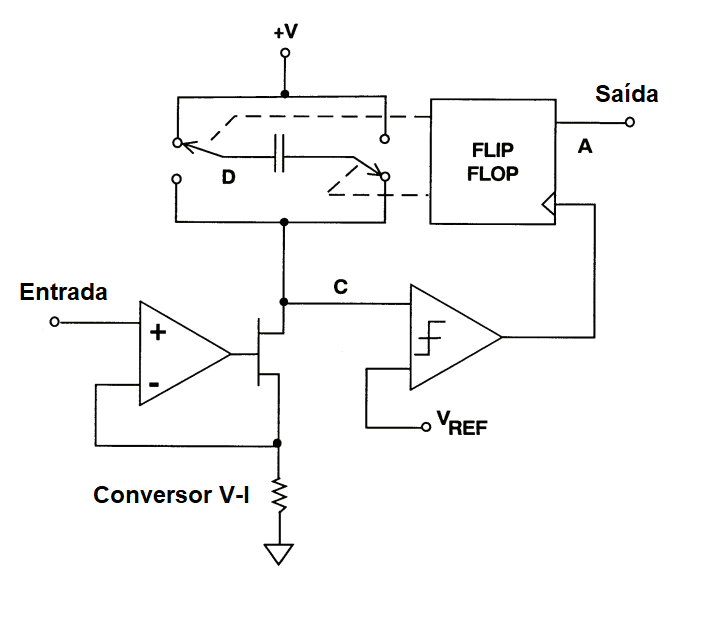
\includegraphics[width=.8\linewidth]{multivibrador.PNG}
  \caption{VFC Multivibrador}
  \label{multivibrador}
  \fonte{\citeonline{handbook}}
\end{minipage}%
\begin{minipage}{.5\textwidth}
  \centering
  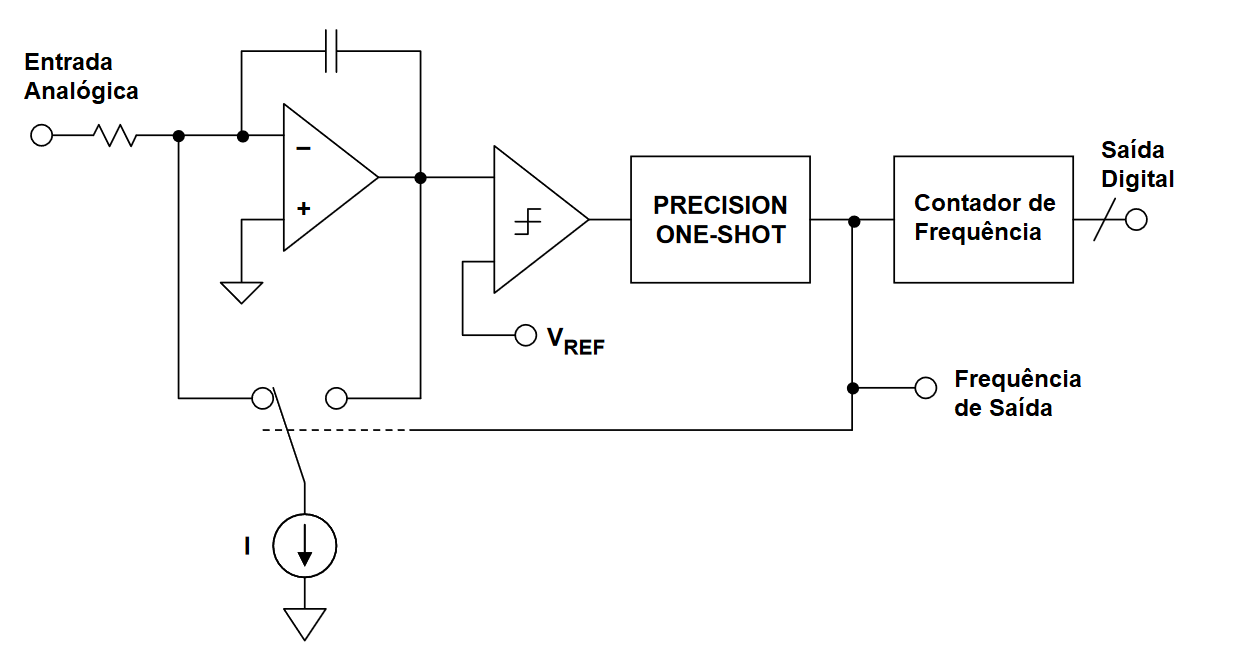
\includegraphics[width=.68\linewidth]{chargebalance.PNG}
  \caption{\textit{Charge-balance VFC}}
  \fonte{\citeonline{handbook}}
  \label{chargebalance}
\end{minipage}
\end{figure}

Este trabalho será focado no VFC multivibrador, por 
\begin{citacao}
possuir acurácia moderada, a qual é boa o suficiente para a aplicação [em WSNs] e ser mais simples do que o \textit{charge-balance VFC}, o que significa melhor compatibilidade para baixo consumo e baixa potência \cite{VFCbook}.
\end{citacao}

\section{VFC Multivibrador}
Este tipo de conversor opera integrando alternadamente uma tensão de entrada e gerando pulsos quando a saída do integrador se igualar a uma tensão de referência \cite{kirianaki}. A figura \ref{modeloVFC} apresenta a estrutura desse circuito.

\begin{figure}[!ht]
  \centering
  % Requires \usepackage{graphicx}
  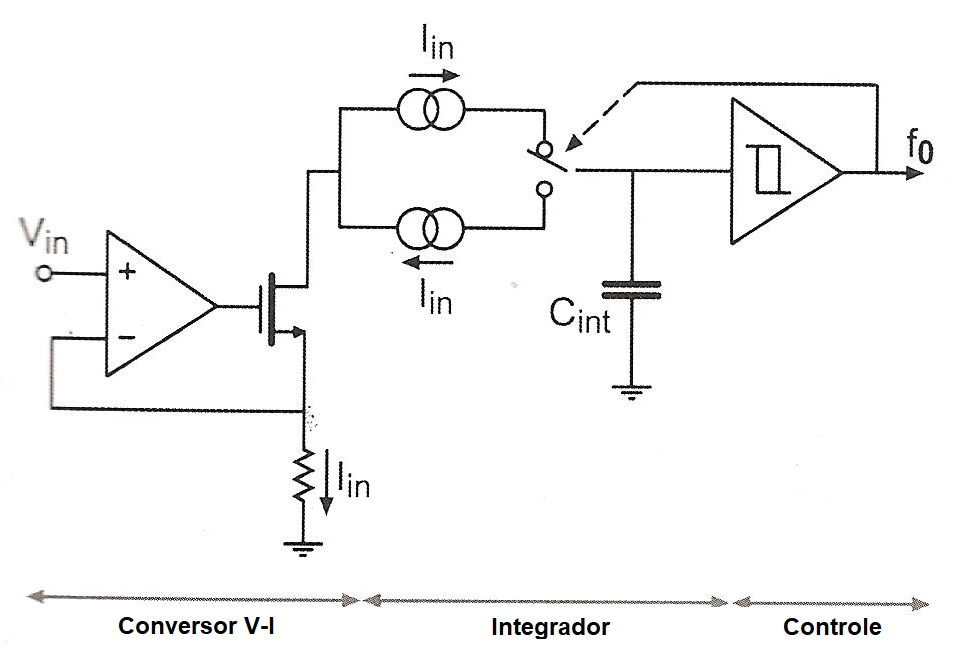
\includegraphics[width=300pt]{modeloVFC.png}\\
  \caption{Implementação típica de um VFC multivibrador}\label{modeloVFC}
  \fonte{\citeonline{VFCbook}}
\end{figure}

Conforme observado por \citeonline{handbook}:
\begin{citacao}
O VFC multivibrador é, na verdade, um conversor de corrente-frequência \verb|[...]|, porém, na prática os circuitos contém um conversor tensão-corrente na entrada. \verb|[...]| a corrente descarrega o capacitor até que um limite inferior seja atingido, e quando os terminais do capacitor são revertidos, o meio-ciclo se repete.
\end{citacao}

Da figura \ref{modeloVFC}, tem-se que um VFC multivibrador é composto por três blocos: um conversor tensão-corrente na entrada, um integrador de corrente bidirecional e um circuito de controle retroalimentado com o integrador. Tem-se então o seguinte princípio de operação: Uma corrente de entrada \(I_{in}\), obtida através da conversão de uma tensão de entrada \(V_{in}\), carrega e descarrega um capacitor \(C_{int}\) entre dois limites, \(V_{H}\) e \(V_{L}\), estabelecidos pelo circuito de controle. O integrador gera uma forma de onda triangular, a qual se transforma em uma onda quadrada ao passar pelo circuito de controle. Esta onda de saída atua tanto fornecendo a frequência de saída do VFC quanto controlando, retroativamente, o integrador \cite{VFCbook}.

\begin{figure}[!ht]
  \centering
  % Requires \usepackage{graphicx}
  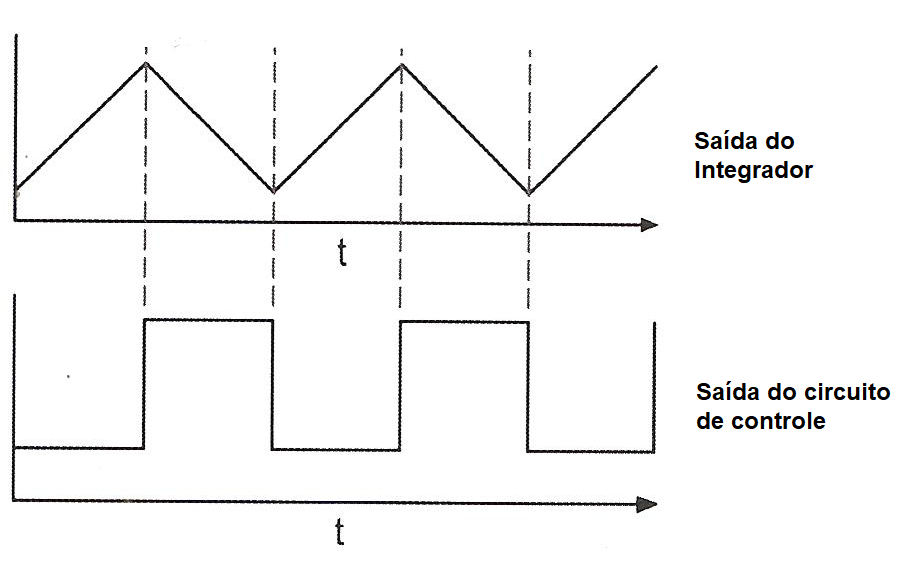
\includegraphics[width=300pt]{VFCOndas.png}\\
  \caption{Tensões de saída}\label{VFCOndas}
  \fonte{\citeonline{VFCbook}}
\end{figure}

As tensões de saída do integrador e do circuito de controle (a qual também é a tensão de saída do próprio VFC) são mostradas na figura \ref{VFCOndas}.

As seguintes subseções deste capítulo abordam os três blocos que formam um conversor tensão-frequência multivibrador.

\subsection{Conversor tensão-corrente}

Uma das formas de se converter uma tensão de entrada em corrente baseia-se no uso de um Amplificador Operacional de Transcondutância (OTA) energizando um MOSFET e um resistor aterrado em uma configuração de feedback negativo. A figura \ref{conversorvi} mostra uma implementação dessa estrutura com a adição de uma bateria flutuante cujo objetivo é escalar a tensão de saída VA em um fator $\alpha$, sendo $0 < \alpha < 1$. Dessa forma, o transistor T1 estará atuando sempre em saturação, o que permite o funcionamento rail-to-rail.

\begin{figure}[!ht]
  \centering
  % Requires \usepackage{graphicx}
  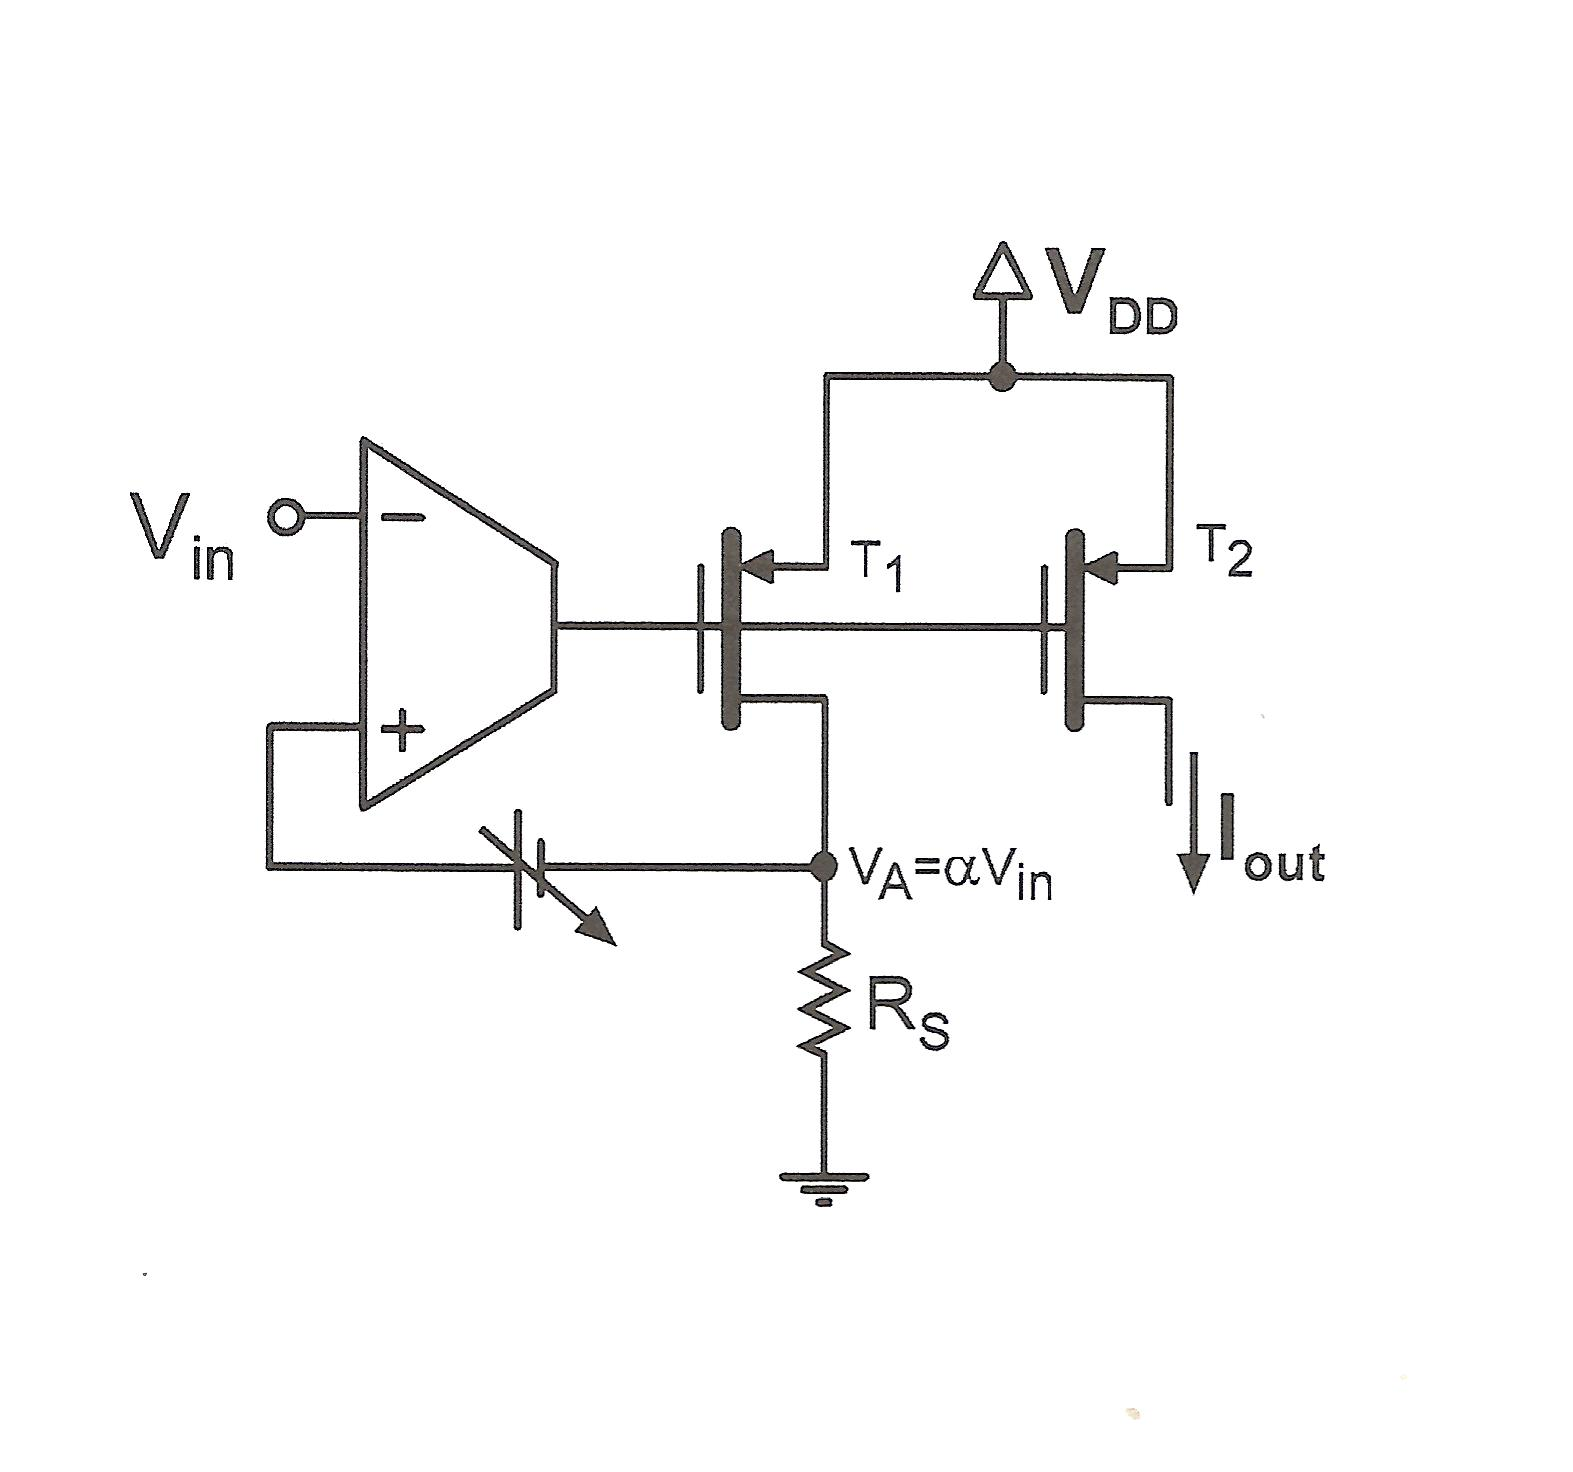
\includegraphics[width=300pt]{conversorvi.png}\\
  \caption{Esquema para conversor V-I \textit{rail-to-rail}}\label{conversorvi}
  \fonte{\citeonline{VFCbook}}
\end{figure}

Dado este modelo, o fator de atenuação $\alpha$ pode ser implementado de diversas maneiras. \textit{Feedforward   voltage   attenuation} (FFVA), \textit{feedback voltage attenuation} (FBVA) e \textit{current attenuation} (CA) são três abordagens comuns \cite{azcona-calvo} ilustradas nas figuras \ref{ffva}, \ref{fbva} e \ref{ca}, respectivamente.

\begin{figure}[H]
\centering
\begin{minipage}{.5\textwidth}
  \centering
  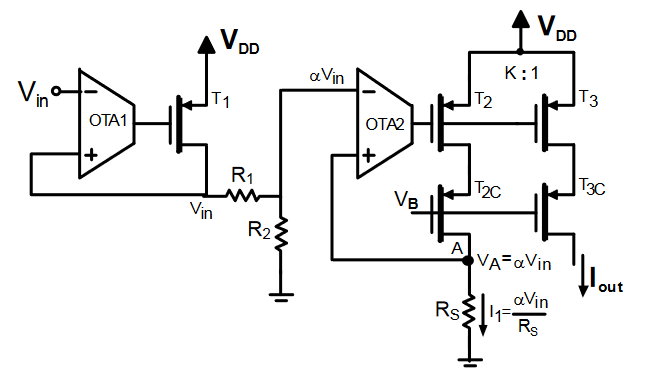
\includegraphics[width=.6\linewidth]{ffva.PNG}
  \caption{FFVA}
  \label{ffva}
  \fonte{\citeonline{azcona-calvo}}
\end{minipage}%
\begin{minipage}{.5\textwidth}
  \centering
  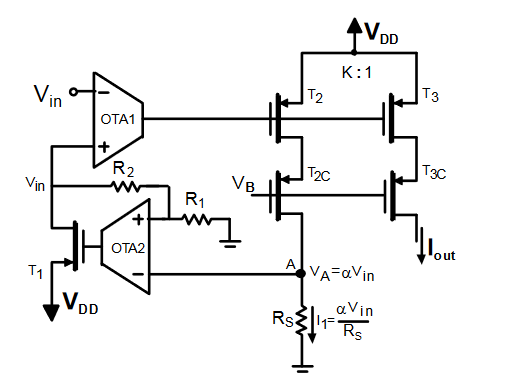
\includegraphics[width=.68\linewidth]{fbva.PNG}
  \caption{FBVA}
  \fonte{\citeonline{azcona-calvo}}
  \label{fbva}
\end{minipage}
\begin{minipage}{.5\textwidth}
  \centering
  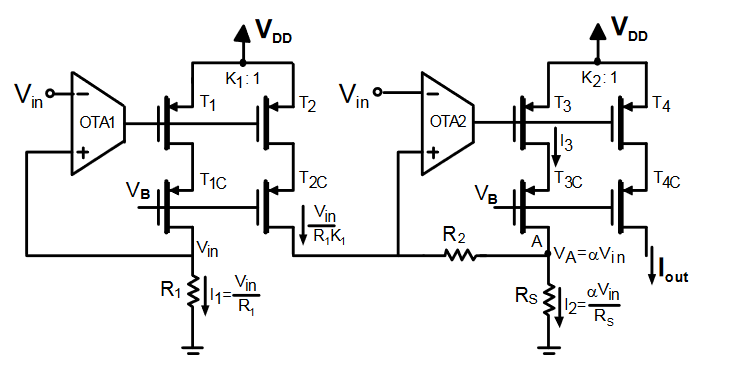
\includegraphics[width=.68\linewidth]{ca.png}
  \caption{CA}
  \fonte{\citeonline{azcona-calvo}}
  \label{ca}
\end{minipage}
\end{figure}

Neste trabalho, será utilizada a arquitetura FFVA, por ser a mais simples das três, possuindo baixo consumo de energia enquanto mantém a faixa de entrada alta, e atender às especificações do projeto.

\subsubsection{OTA}
Nesta seção, inicialmente serão discutidos brevemente alguns princípios de operação e blocos que compõem um amplificador operacional simples. Em seguida, diferentes topologias serão analisadas. Finalmente, circuitos para operação \textit{rail-to-rail} serão estudados.

\subsubsubsection{Espelhos de Corrente}
O espelho de corrente é um dos blocos fundamentais no projeto de circuitos integrados. "A principal propriedade dessa topologia é que ela permite copiar precisamente uma corrente de forma independente de processo e de temperatura" \cite{razavi}. Através de espelhos de corrente, uma corrente de referência pode ser replicada conforme o necessário no projeto de um circuito.

\begin{figure}[!ht]
  \centering
  % Requires \usepackage{graphicx}
  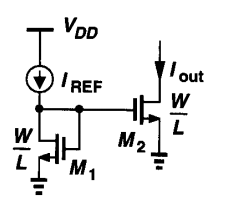
\includegraphics[width=200pt]{espelho.PNG}\\
  \caption{Espelho de corrente simples}\label{espelhoSimples}
  \fonte{\citeonline{razavi}}
\end{figure}

A chave para o funcionamento deste circuito está na relação entre os transistores M1 e M2 (figura \ref{espelhoSimples}), que faz com que a corrente de saída seja dada pela equação \ref{eqEspelho} \cite{razavi}:

\begin{equation}\label{eqEspelho}
I_{out} = \frac{(W/L)_2}{(W/L)_1}I_{REF}
\end{equation}

Esta relação, no entanto, foi obtida através de equações simplificadas que desconsideram o efeito de modulação de canal nos transistores. Na prática, a cópia feita por um espelho simples não é tão precisa. Para resolver esse problema, pode-se utilizar a estrutura do espelho de corrente \textit{cascode}. Além de permitir uma cópia mais precisa da corrente de referência, a estrutura \textit{cascode} também aumenta a resistência de saída do circuito, tornando-o assim mais próximo de uma fonte de corrente ideal.

O problema dessa abordagem, no entanto, está no consumo substancial de \textit{headroom} imposto pelo transistor M3 (figura \ref{espelho}). Uma maneira de minimizar este problema é mostrada na figura \ref{cascodeEspelhoWide}. Este circuito, denominado espelho de corrente de amplo alcance \cite{razavi}, aumenta o \textit{headroom} do espelho \textit{cascode} com o custo de necessitar de um circuito extra de polarização para prover a tensão \(V_b\).

\begin{figure}[H]
\centering
\begin{minipage}{.5\textwidth}
  \centering
  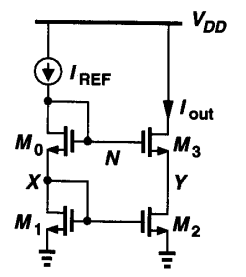
\includegraphics[width=.6\linewidth]{cascodeEspelho.PNG}
  \caption{Espelho de corrente cascode}
  \label{espelho}
  \fonte{\citeonline{razavi}}
\end{minipage}%
\begin{minipage}{.5\textwidth}
  \centering
  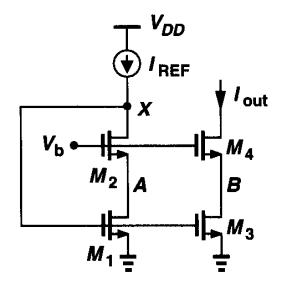
\includegraphics[width=.68\linewidth]{cascodeEspelhoWide.PNG}
  \caption{Espelho de corrente cascode de amplo alcance}
  \fonte{\citeonline{razavi}}
  \label{cascodeEspelhoWide}
\end{minipage}
\end{figure}

\subsubsubsection{Par diferencial}
Assim como num amplificador operacional convencional, um OTA atua amplificando um sinal diferencial. Isso ocorre mesmo em aplicações que requerem a amplificação de uma única tensão, pois na maioria desses casos o amplificador estará operando com retroalimentação negativa.
"O amplificador diferencial está entre as invenções mais importantes envolvendo circuitos \verb|[...]|; oferecendo muitas propriedades úteis, a operação diferencial se tornou a escolha dominante nos circuitos de sinal analógico ou mistos na atualidade." \cite{razavi}

A forma mais comum de se amplificar um sinal diferencial é através do par diferencial, que é o bloco de entrada da grande maioria dos circuitos de amp ops e OTAs e, portanto, muitas propriedades de um \textit{amp op} dependem dos parâmetros desse bloco \cite{dehghani2013design}. A figura \ref{parDiff} mostra um par diferencial simples.
\begin{figure}[!ht]
  \centering
  % Requires \usepackage{graphicx}
  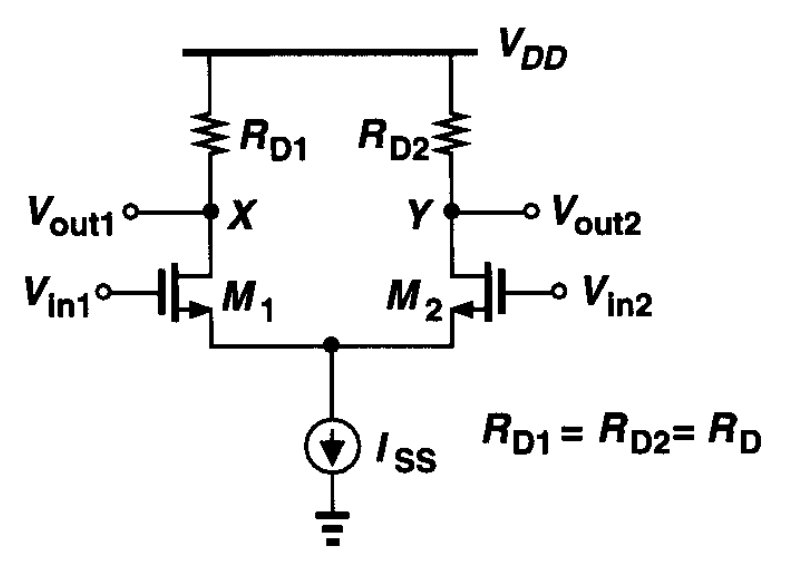
\includegraphics[width=200pt]{parDiff.PNG}\\
  \caption{Par diferencial básico}\label{parDiff}
  \fonte{\citeonline{razavi}}
\end{figure}

\subsubsubsection{Topologia folded cascode}
Generalizando da forma mais superficial possível, toda a operação de um amplificador operacional nada mais é do que uma tensão diferencial de entrada que é convertida para uma corrente equivalente pelo par diferencial, a qual flui por um elemento de alta impedância, geralmente uma carga ativa, para converter novamente a corrente em uma tensão de maior amplitude \cite{dehghani2013design}.

A partir daí, estágios adicionais podem ser cascateados para proverem benefícios extras, como aumento de ganho e diminuição da impedância de saída, por exemplo. À partir desse princípio, derivam-se muitas topologias de amplificadores diferenciais, como o amplificador de dois estágios (figura \ref{twoStage}), o amplificador \textit{telescopic cascode} (figura \ref{telescopic}) e o \textit{folded cascode} (figura \ref{folded}).

\begin{figure}[H]
\centering
\begin{minipage}{.5\textwidth}
  \centering
  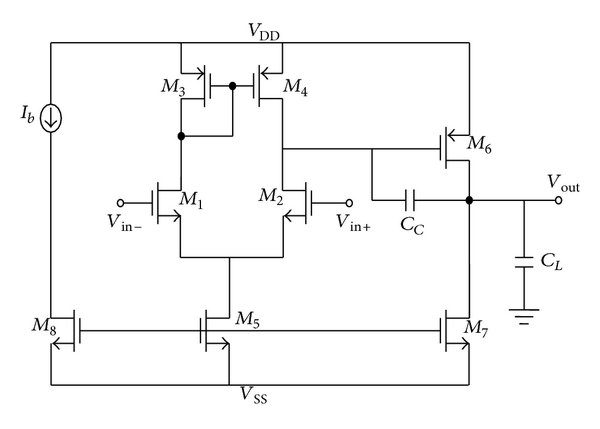
\includegraphics[width=.8\linewidth]{twoStage.jpg}
  \caption{Amplificador diferencial de dois estágios}
  \label{twoStage}
  \fonte{\citeonline{twoStage}}
\end{minipage}%
\begin{minipage}{.5\textwidth}
  \centering
  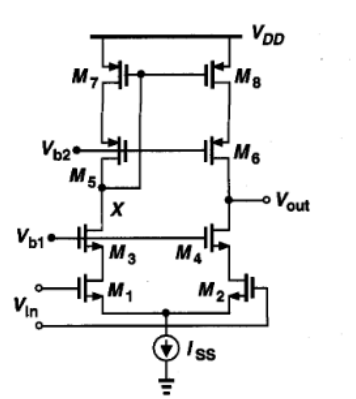
\includegraphics[width=.68\linewidth]{telescopic.PNG}
  \caption{Telescopic cascode}
  \fonte{\citeonline{razavi}}
  \label{telescopic}
\end{minipage}
\end{figure}

A topologia escolhida para o OTA a compor o VFC deste trabalho foi a \textit{folded cascode}. Essa estrutura, apesar de prover menos ganho do que o amplificador de dois estágios, possui a vantagem de não necessitar de compensação de frequência através de capacitores, além de possuir o mesmo ganho e resposta em frequência do telescopic cascode, porém com a vantagem de uma maior excursão de saída em relação a esse último quando usada como seguidor de tensão \cite{dehghani2013design}.

Conforme escrito por \citeonline{razavi}: "A ideia de uma estrutura \textit{cascode} é converter a tensão de entrada em uma corrente e aplicar o resultado a um estágio \textit{commom-gate}". No caso do \textit{folded cascode}, são usados transistores de tipos diferentes para o par de entrada e o estágio \textit{cascode}.

Em um amplificador desse tipo, o par diferencial de entrada possui como carga ativa um espelho de corrente de amplo alcance, sendo que o estágio \textit{common gate} age como um \textit{buffer} de corrente e é o responsável por injetar a corrente diferencial do par de entrada na carga. A Figura \ref{folded} mostra a estrutura, na qual os transistores PMOS M6 e M7 agem como os transistores cascode para o par NMOS M1 e M2.

\begin{figure}[!ht]
  \centering
  % Requires \usepackage{graphicx}
  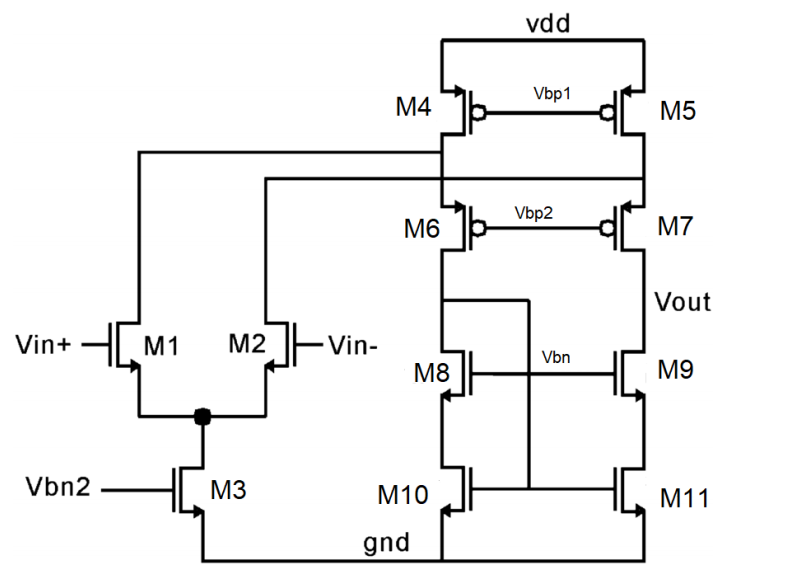
\includegraphics[width=300pt]{folded.PNG}\\
  \caption{Topologia \textit{folded cascode} utilizando um espelho de corrente de amplo alcance}\label{folded}
  \fonte{\citeonline{dehghani2013design}}
\end{figure}

Segundo \citeonline{dehghani2013design}, esta estrutura é ideal para operar com cargas capacitivas altas, pois um aumento da capacitância da carga resulta em um aumento da estabilidade do amplificador, com o custo de uma redução da largura de banda.

\subsubsubsection{Operação rail-to-rail e circuitos para transcondutância constante}
O alcance da excursão do sinal de entrada do amplificador é um parâmetro crítico para o funcionamento do VFC proposto, visto que ele também corresponde ao alcance do conversor.
Portanto, é imperativo que este amplificador opere com tensão de entrada \textit{rail-to-rail}. Conforme argumentam \citeonline{VFCbook}:
\begin{citacao}
\verb|[...]| caso esta característica não seja atingida [funcionamento \textit{rail-to-rail}], haverá perda na relação sinal-ruído (SNR) do VFC. Consequentemente, nós não poderemos aproveitar a máxima sensibilidade da conversão frequência-para-código DCM subsequente e, para uma determinada janela \(T_W\), resolução efetiva será perdida.  
\end{citacao}
Dadas estas motivações, surge a necessidade do projeto de um estágio de entrada \textit{rail-to-rail}, e a forma mais simples de se obter esta característica é utilizando-se dois pares diferenciais em paralelo, sendo um de transistores NMOS e outro, PMOS, conforme mostrado na figura \ref{pares-paralelos}.

\begin{figure}[H]
\centering
\begin{minipage}{.4\textwidth}
  \centering
  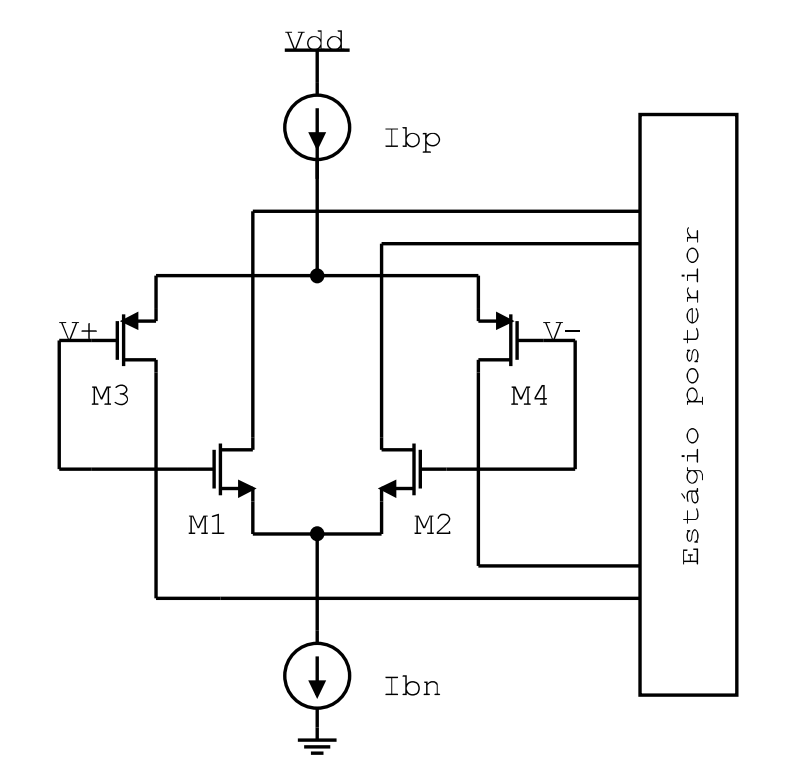
\includegraphics[width=.8\linewidth]{pares-paralelos.png}
  \caption{Estágio de entrada com pares diferenciais complementares}
  \label{pares-paralelos}
  \fonte{\citeonline{Leandro}}
\end{minipage}%
\begin{minipage}{.6\textwidth}
  \centering
  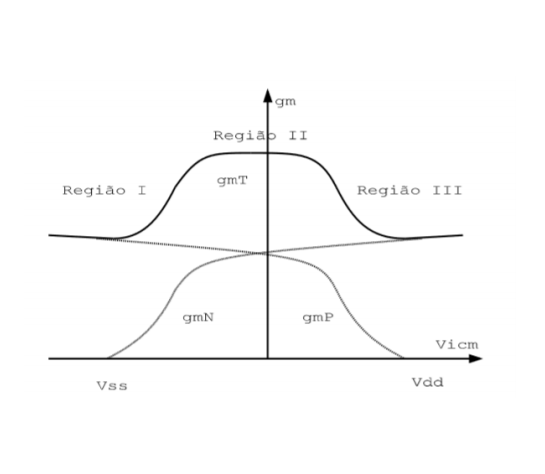
\includegraphics[width=.8\linewidth]{transconductanceRails.PNG}
  \caption{Variação da transcondutância}
  \fonte{\citeonline{Leandro}}
  \label{transconductanceRails}
\end{minipage}
\end{figure}

Um par diferencial NMOS, ao ter sua entrada negativa curto-circuitada com a saída, tem sua tensão de saída mínima limitada inferiormente, devido ao transistor que implementa a fonte de corrente polarizando o par entrar em triodo. Ou seja, a tensão de entrada em modo comum mínima é limitada por \(V_{icm,min} = V_{GSn} + V_{od,I_{SS}}\) (onde \(V_{GSn}\) corresponde à tensão porta-fonte nos transistores do par e \(V_{od,I_{SS}}\) à sobretensão de condução do transistor atuando como fonte de corrente), enquanto que \(V_{ic,max}\) pode variar próximo a $V_{DD}$. 

Por outro lado, para o par diferencial PMOS o oposto acontece, podendo a tensão modo comum de entrada variar próxima de zero porém sendo limitada superiormente por \(V_{icm,max} = V_{DD} + V_{GSp} - V_{od,I_{SS}}\).

Portanto, justifica-se o uso dos dois pares em paralelo. Deste modo, ao menos um dos pares estará funcionando por toda a excursão do sinal de entrada. Como é de costume no \textit{design} de circuitos, no entanto, existe uma relação de compromisso. Nesse caso, a operação \textit{rail-to-rail} vem com o custo de afetar a transcondutância do circuito. A variação da transcondutância total desse estágio de entrada é mostrada na Figura \ref{transconductanceRails}.

Desse modo, definem-se três regiões \cite{Leandro}:
\begin{itemize}
    \item Região I: $V_{icm} \sim  0$: apenas o par PMOS conduz e o par NMOS encontra-se
desligado.
    \item Região II: $V_{icm} \sim V_{DD}/2$: ambos os pares conduzem.
    \item Região III: $V_{icm} \sim V_{DD}$: apenas o par NMOS conduz e o par PMOS encontra-se desligado.
\end{itemize}

Observa-se que há um aumento significativo na transcondutância total na região 2,
quando ambos os pares conduzem. Essa variação na transcondutância tem efeito sobre o
ganho, a margem de ganho e fase e muito possivelmente causa instabilidade \cite{dehghani2013design}.

\subsubsubsection{Circuitos para transcondutância constante}
Dadas as consequências da variação da transcondutância total em um amplificador, é imperativo que se inclua um circuito extra que trabalhe de forma a manter esta transcondutância o mais constante possível.

Neste trabalho será considerado que os transistores NMOS estão apropriadamente
casados com os transistores PMOS, ou seja, \(K_n = \frac{1}{2}\mu_{n}C_{ox}(\frac{W}{L})_n(\Delta V_{GS})^2 = K_p = \frac{1}{2}\mu_{p}C_{ox}(\frac{W}{L})_p(\Delta V_{GS})^2 = K\).

Um modo de se atingir transcondutância constante é utilizar um circuito que se aproveita da relação
quadrática da corrente de dreno nos MOSFETS, exemplificado na figura \ref{hogervorstCircuit}, que atua adicionando uma corrente de $3I_{ss}$ a $I_{ss}$ nas fontes dos transistores do par PMOS quando a tensão de modo comum de entrada está próxima de zero e nas fontes dos transistores do par NMOS quando \(V_{icm} ~ \approx V_{DD}\). Quando $V_{icm}$ está entre esses dois extremos nenhuma corrente é adicionada \cite{hogervorst}.

\begin{figure}[!ht]
  \centering
  % Requires \usepackage{graphicx}
  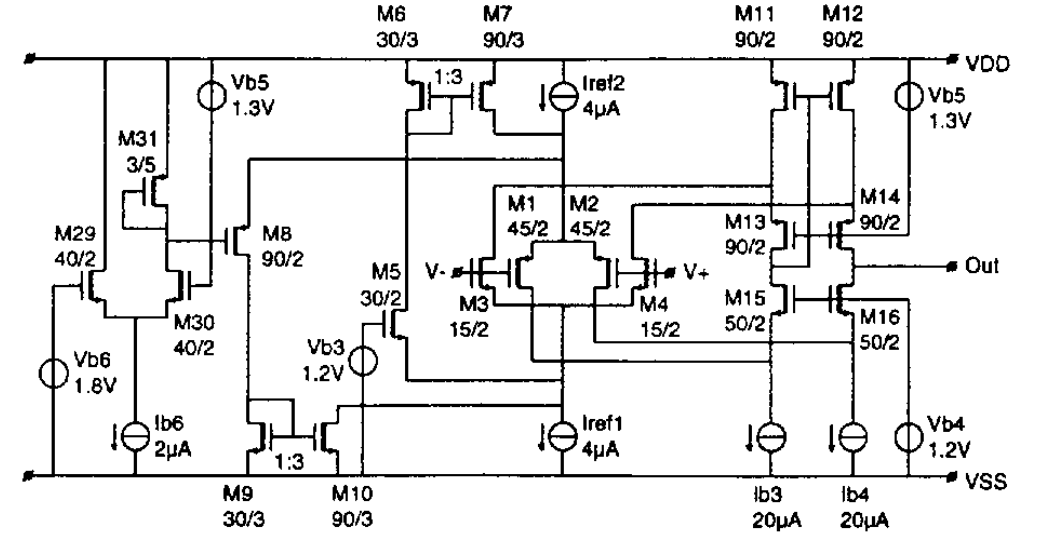
\includegraphics[width=300pt]{hogervorstCircuit.PNG}\\
  \caption{Alternativa para circuito de transcondutância constante}\label{hogervorstCircuit}
  \fonte{\citeonline{hogervorst}}
\end{figure}

Outra forma, muito mais simples, proposta por \citeonline{Minsheng} e mostrada na figura \ref{deslocadores}, utiliza quatro transistores para deslocar o nível de transcondutância de um dos pares diferenciais, de forma que com isso a soma se mantenha constante, conforme mostra a figura \ref{overlap}.
O valor \(\Delta V_{optimal}\) para o deslocamento de nível foi definido pela equação \ref{eqDesloca} \cite{Minsheng}:

\begin{equation}\label{eqDesloca}
2V_{GMBn} < \Delta V_{optimal} < 2V_{GMBn}+\sqrt{\frac{I_{sn0}}{K_{M1}}}
\end{equation}

\begin{figure}[!ht]
  \centering
  % Requires \usepackage{graphicx}
  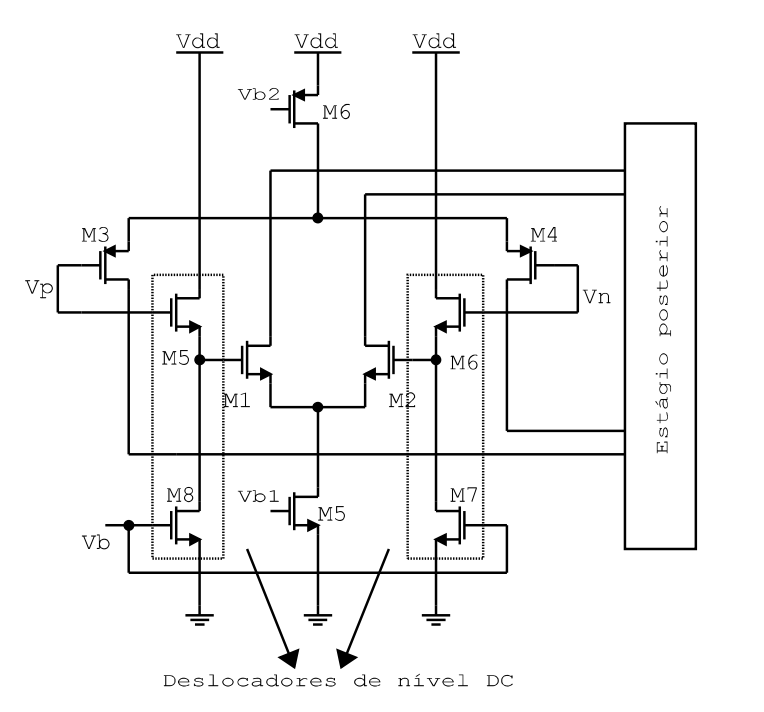
\includegraphics[width=300pt]{deslocadores.PNG}\\
  \caption{Circuito com deslocadores de nível}\label{deslocadores}
  \fonte{\citeonline{Leandro}}
\end{figure}

\begin{figure}[!ht]
  \centering
  % Requires \usepackage{graphicx}
  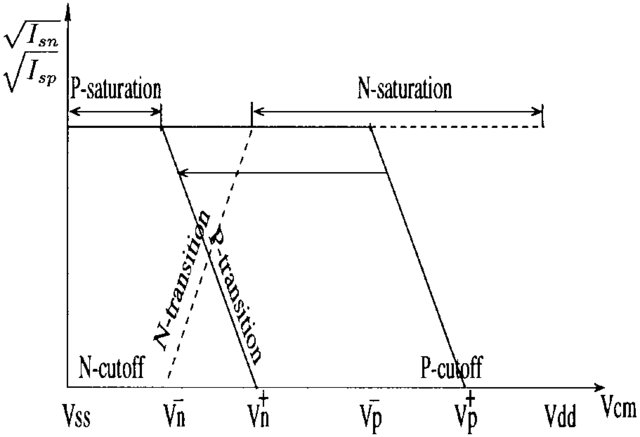
\includegraphics[width=300pt]{overlap.jpg}\\
  \caption{Deslocando a curva de transcondutância}\label{overlap}
  \fonte{\citeonline{Minsheng}}
\end{figure}

\subsubsection{FFVA}
Esta estrutura funciona empregando um divisor de tensão \textit{rail-to-rail} antes do conversor V-I OTA/\textit{common source} principal \cite{azcona-calvo}. Desta forma, a tensão de entrada é atenuada por um fator $\alpha$ de forma que os transistores do estágio \textit{common source} permaneçam em saturação para toda a excursão do sinal de entrada. Da figura \ref{ffva}, tem-se as relações das equações \ref{eqAlfa} e \ref{eqIout}. 
\begin{equation}\label{eqAlfa}
\alpha = \frac{R_2}{R_1 + R_2}
\end{equation}

\begin{equation}\label{eqIout}
I_{out} = \frac{\alpha V_{in}}{KR_{S}}
\end{equation}

\subsection{Integrador de corrente bidirecional}
O próximo bloco a compor a cadeia de circuitos que formará o VFC multivibrador objeto de estudo deste trabalho é um integrador de corrente bidirecional. Segundo \citeonline{VFCbook}, "\verb|[...]| também conhecido como circuito de carga/descarga, [este circuito] consiste em um capacitor \(C_{int}\), uma fonte de corrente que carrega o capacitor e outra que o descarrega".

O processo de carga e descarga do capacitor é controlado por um circuito de controle (que será discutido na próxima seção) que estabelece os limites \(V_{H}\) e \(V_{L}\), de forma que cada vez que a tensão do capacitor atinge um destes limites, a fase de carga do mesmo é revertida.

Deste modo, o resultado esperado é que a forma de onda da tensão de saída no capacitor seja triangular, pois a tensão através do capacitor em um dado momento é dada pela equação \ref{eqCap}
\begin{equation}\label{eqCap}
V_{cap}(t) = V_0 + I_t/C_{int}
\end{equation}
O tempo necessário para carga e descarga do capacitor entre os limites de tensão estabelecidos pelo controlador será dado pela equação \ref{eqTempo}, onde \(T\) é o período do sinal triangular \cite{VFCbook}.

\begin{equation}\label{eqTempo}
t = \frac{T}{2} + \frac{C_{int}(V_{H} - V_{L})}{I}
\end{equation}

O esquema da figura \ref{integrador} ilustra um integrador de corrente bidirecional de baixo consumo. Este é definido como de baixo consumo pois exige menos corrente da fonte para seu funcionamento em relação a um integrador tradicional. Nele, o espelho de corrente de amplo alcance ilustrado age tanto para carregar, quanto para descarregar o capacitor \(C_{int}\). Os transistores \(S_{DW}\) e \(S_{UP}\) agem como \emph{switches} controlados pelo circuito de controle do próximo estágio, definindo os momentos de carga e descarga.

\begin{figure}[!ht]
  \centering
  % Requires \usepackage{graphicx}
  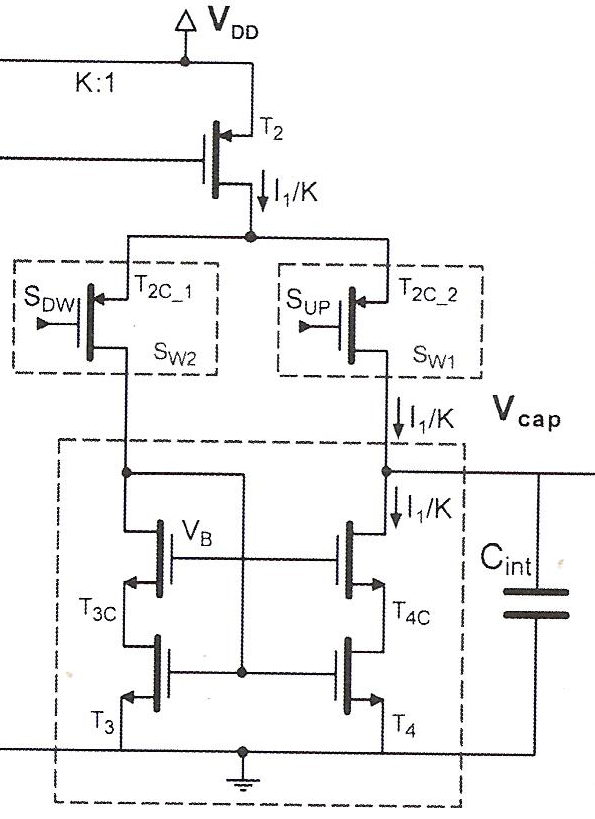
\includegraphics[width=200pt]{integrador.png}\\
  \caption{Integrador de corrente bidirecional de baixo consumo}\label{integrador}
  \fonte{\citeonline{VFCbook}}
\end{figure}

\subsection{Circuito de controle}

Conforme discutido anteriormente, o circuito de controle, último dos três blocos principais de um VFC, é o responsável por prover tanto o sinal digital que liga/desliga os transistores \(SW_1\) e \(SW_2\) (figura \ref{integrador}) quanto a saída do VFC em si. Dentre os circuitos de controle mais utilizados para a aplicação em questão estão os \textit{voltage window comparators} (VWC) e o disparador Schmitt.
Este último no entanto, por ser um comparador com uma histerese inerente, é fortemente dependente de variações em temperatura e fonte \cite{VFCbook}, sendo então o VWC o circuito mais indicado para o VFC.
A figura \ref{VWC} apresenta o diagrama de blocos de um comparador VWC e a tabela \ref{tabFlipFlop} mostra a operação do circuito.

\begin{figure}[!ht]
  \centering
  % Requires \usepackage{graphicx}
  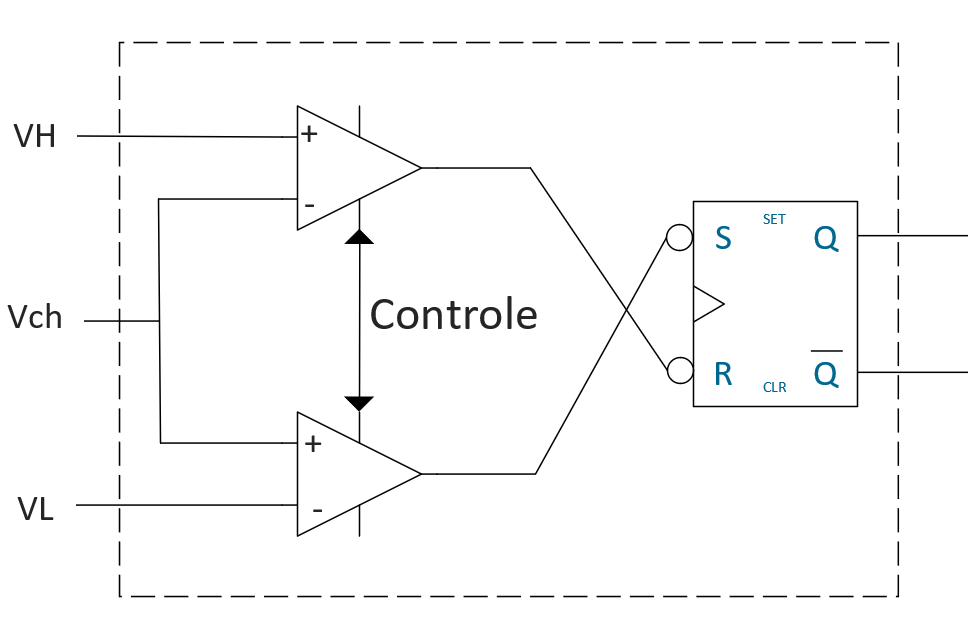
\includegraphics[width=300pt]{VWC.PNG}\\
  \caption{VWC implementado com dois comparadores e um \textit{flip-flop} RS}\label{VWC}
\end{figure}

\begin{table}[h]
    \begin{center}    
    \begin{tabular}{ | c | c | c | c | }
    \hline
    \(V_{cap}\) & \(\overline{S}\) & \(\overline{R}\) & Q \\ 
    \hline
    - & 0 & 0 & 0 \\ 
    \hline
    \(V_{cap} \leq V_{L}\) & 0 & 1 & 1 \\ 
    \hline
    \(V_{cap} \geq V_{H}\) & 1 & 0 & 0 \\ 
    \hline
    \(V_{L} \leq V_{cap} \leq V_{H}\) & 1 & 1 & Q anterior \\
    \hline
    \end{tabular}
    \caption[Operação do VWC]{Operação do VWC }
    \label{tabFlipFlop}
    \end{center}
\end{table}

O esquema completo do VFC a ser projetado é mostrado na figura \ref{VFC_final}.

\begin{figure}[!ht]
  \centering
  % Requires \usepackage{graphicx}
  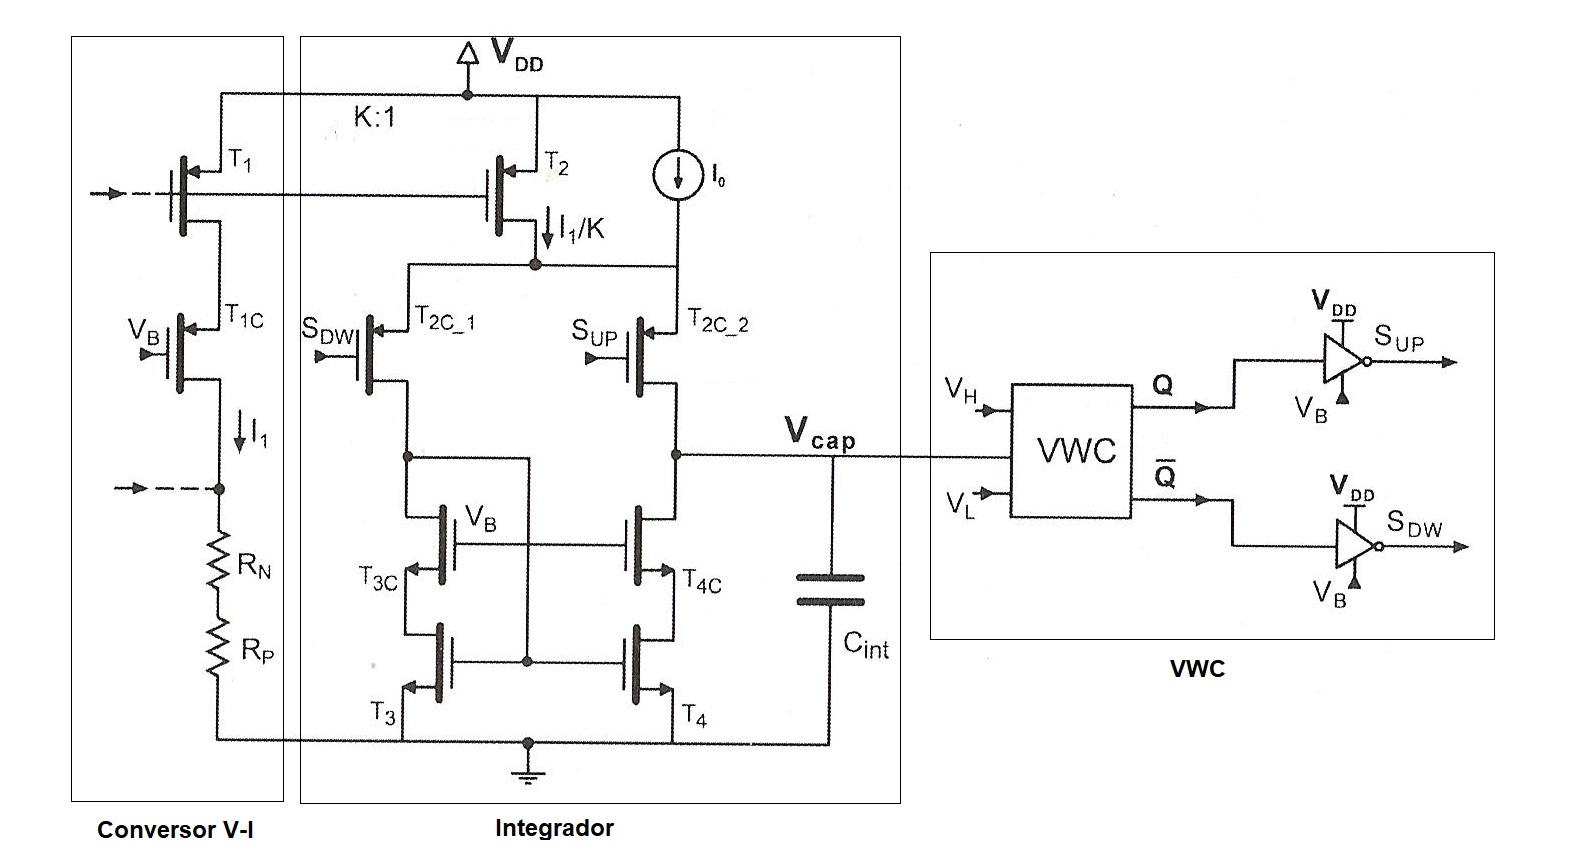
\includegraphics[width=300pt]{VFC_final.jpeg}\\
  \caption{VFC}\label{VFC_final}
  \fonte{Adaptado de \citeonline{VFCbook}}
\end{figure}

% ----------------------------------------------------------------
% Metodologia *******************
% ----------------------------------------------------------------
\chapter{Metodologia}

\section{Obtenção dos parâmetros dos transistores utilizados}

Antes de se iniciar o projeto, é necessário estimar-se alguns parâmetros dos
transistores NMOS e PMOS para que estes possam ser utilizados nos cálculos das equações. Neste trabalho serão utilizados transistores de tecnologia IBM 130nm. As figuras \ref{testeNMOS} e \ref{testePMOS} mostram os circuitos de teste desenhados no software Cadence Virtuoso e a figura \ref{curvaN} exemplifica a saída da simulação para o transistor NMOS. Através da simulação DC no simulador Spectre, obteve-se os parâmetros para os transistores que constam na tabela \ref{tabTrans}.

\begin{figure}[H]
\centering
\begin{minipage}{.5\textwidth}
  \centering
  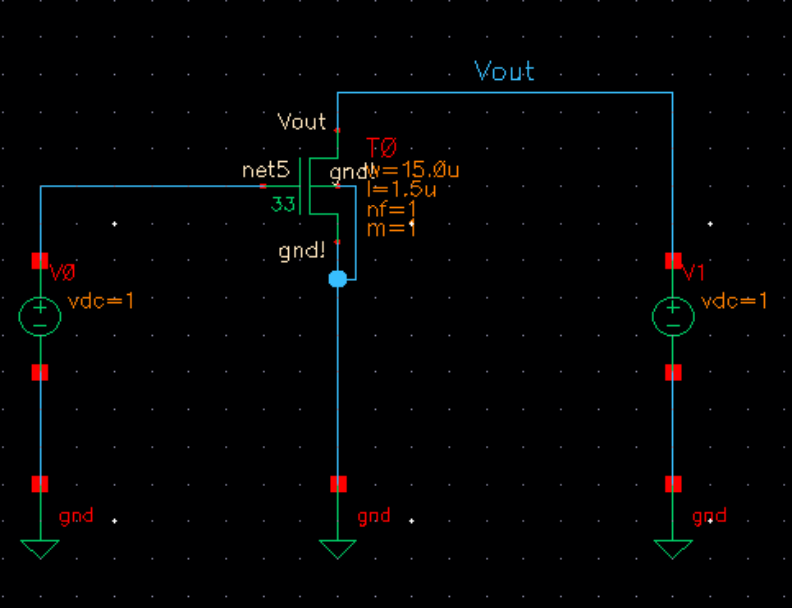
\includegraphics[width=.8\linewidth]{nmos.PNG}
  \caption{Simulação NMOS}
  \label{testeNMOS}
\end{minipage}%
\begin{minipage}{.5\textwidth}
  \centering
  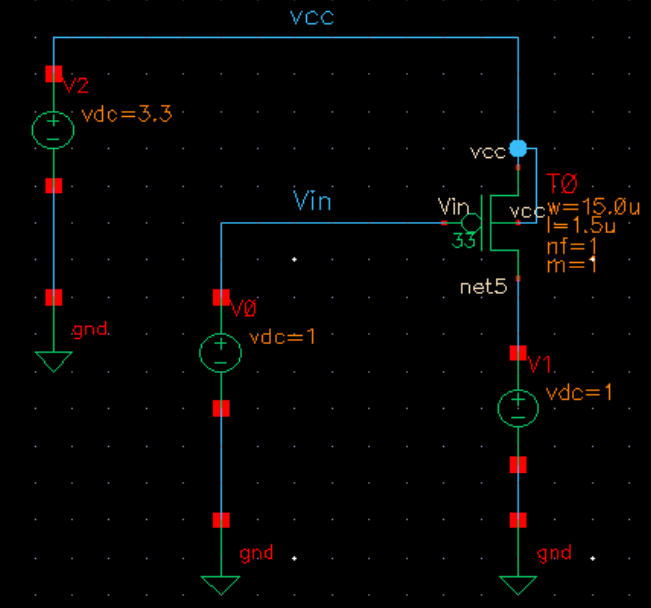
\includegraphics[width=.68\linewidth]{pmos.PNG}
  \caption{Simulação PMOS}
  \label{testePMOS}
\end{minipage}
\end{figure}

\begin{figure}[!ht]
  \centering
  % Requires \usepackage{graphicx}
  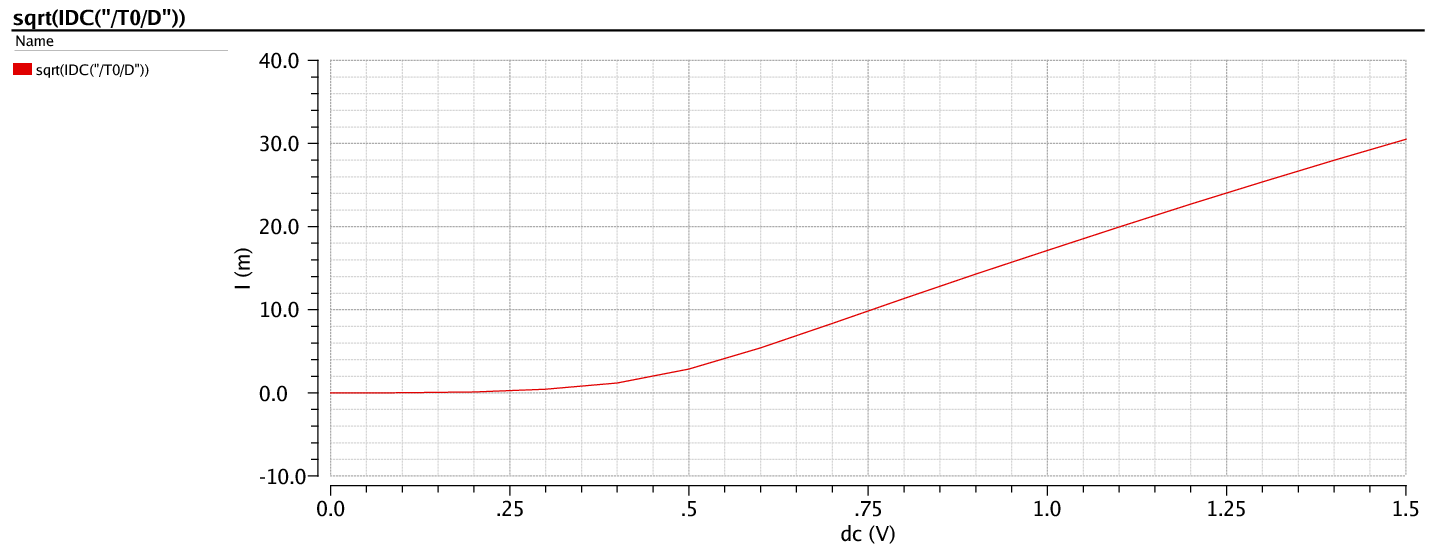
\includegraphics[width=300pt]{paramN.PNG}\\
  \caption{Resultado da simulação DC do transistor NMOS}\label{curvaN}
\end{figure}

\begin{table}[h]
    \begin{center}    
    \begin{tabular}{ | c | c | }
    \hline
    \(V_{THn}\) & 460mV \\ 
    \hline
    \(K_n = \frac{1}{2}\mu_{n}C_{ox}\) & $75,88\mu$ \\ 
    \hline
    \(V_{THp}\) & -415mV \\ 
    \hline
    \(K_p = \frac{1}{2}\mu_{p}C_{ox}\) & $21,88\mu$ \\ 
    \hline
    \(\frac{\mu_{n}}{\mu_{p}}\) & 3,5 \\ 
    \hline
    \end{tabular}
    \caption[Parâmetros dos transistores]{Parâmetros dos transistores}
    \label{tabTrans}
    \end{center}
\end{table}

\section{Projeto conversor V-I}
\subsection{OTA}
Para o bloco de entrada \textit{rail-to-rail} foram utilizados um par diferencial PMOS e um NMOS conectados em paralelo. As correntes de polarização para cada par são obtidas através de um espelho de corrente que replica uma corrente de referência $I_{ref}$. Para manter a transcondutância constante, utilizou-se os transistores T10-T11 e T12-T13 como deslocadores de nível para a entrada do par PMOS.

Já para o estágio \textit{folded cascode} foram utilizados dois espelhos de corrente de amplo alcance, um PMOS e outro NMOS, conectados aos pares diferenciais de entrada. A polarização para o espelho NMOS é obtida do pino Ibias, equanto que a do espelho PMOS é feita utilizando-se o transistor T25.

O circuito do OTA projetado é mostrado na figura \ref{circuitoOTA}.

\begin{figure}[!ht]
  \centering
  % Requires \usepackage{graphicx}
  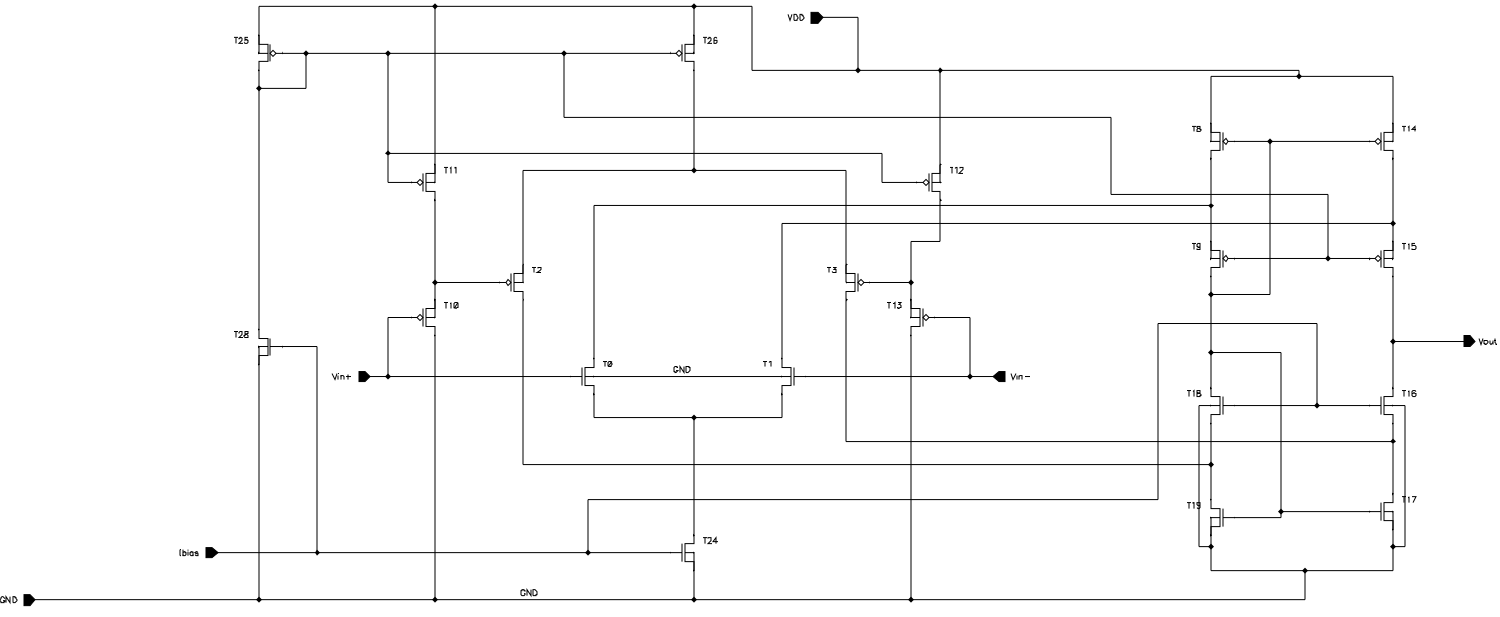
\includegraphics[width=450pt]{circuitoOTA.png}\\
  \caption{Circuito projetado para o OTA \textit{rail-to-rail}}\label{circuitoOTA}
\end{figure}

A tabela \ref{transOTA} mostra as larguras (W) escolhidas para os transistores. O L de todos os transistores foi mantido em $1,5\mu$m para evitar efeitos de modulação de canal.

\begin{table}[h]
    \begin{center}    
    \begin{tabular}{ | c | c | }
    \hline
    T0, T1, T24, T28  & \(15.0 \mu m\) \\ 
    \hline
    T2, T3, T11, T12  & \(20.0 \mu m\) \\ 
    \hline
    T10, T13  & \(70.0 \mu m\) \\ 
    \hline
    T25, T26 & \(52.5 \mu m\) \\ 
    \hline
    T8, T14, T17, T19  & \(3.5 \mu m\) \\ 
    \hline
    T9, T15, T16, T18  & \(1.75 \mu m\) \\ 
    \hline
    \end{tabular}
    \caption[Dimensões dos transistores do OTA]{Dimensões dos transistores do OTA}
    \label{transOTA}
    \end{center}
\end{table}

\subsection{FFVA}

Conforme mencionado anteriormente, a arquitetura escolhida para o conversor V-I foi a FFVA. Na figura \ref{circuitoVI}, \(\mathrm{OTA_{aux}}\) corresponde ao amplificador \textit{folded cascode} \textit{rail-to-rail} projetado anteriormente. Os resistores do FFVA foram dimensionados de forma que $\alpha = 0.5$, possibilitando que o OTA que recebe $\mathrm{V_{in2}}$ fosse implementado com apenas um par diferencial PMOS simples (figura \ref{OTAsimples}), em contraste com o mais complexo \textit{folded cascode} $\mathrm{OTA_{aux}}$. 
A figura \ref{circuitoVI} mostra o circuito e as dimensões e valores dos transistores, resistores e capacitores de compensação utilizados. 

\begin{figure}[!ht]
  \centering
  % Requires \usepackage{graphicx}
  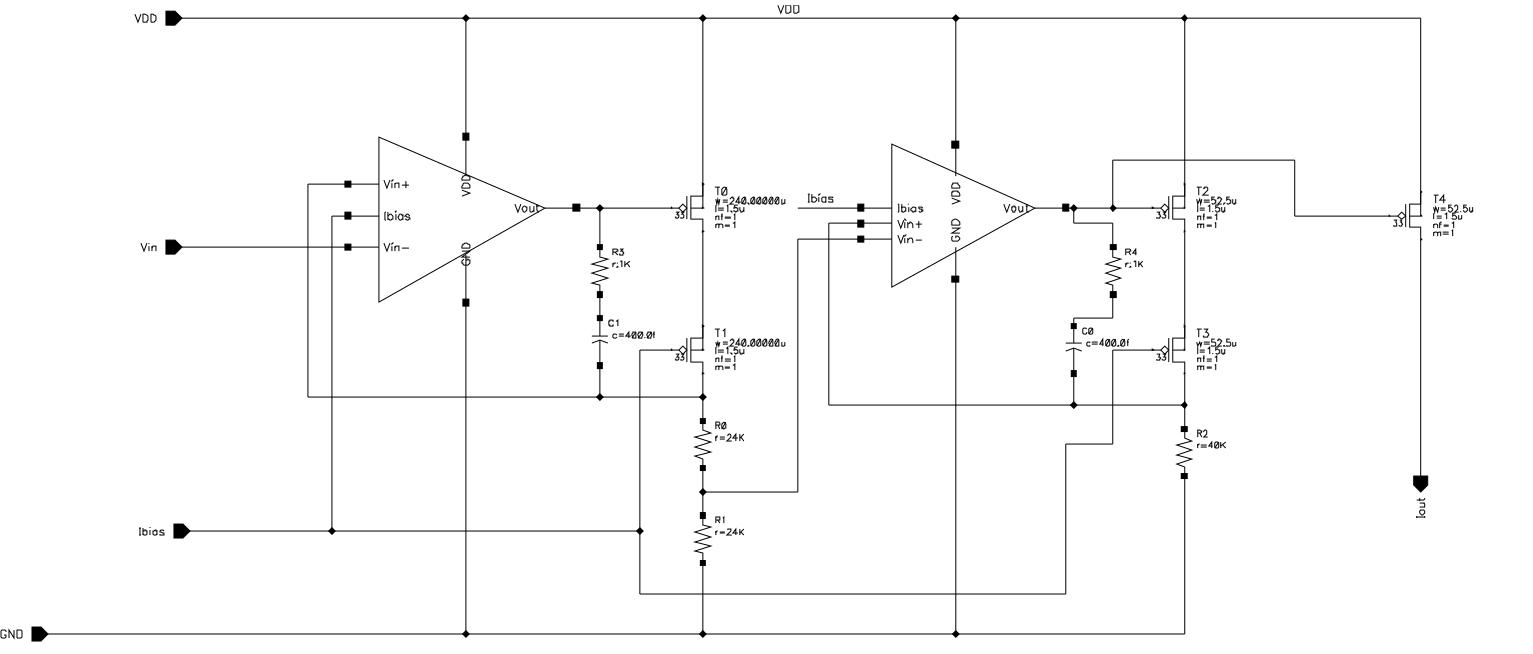
\includegraphics[width=450pt]{circuitoFFVA.png}\\
  \caption{Circuito projetado para o conversor V-I \textit{rail-to-rail}}\label{circuitoVI}
\end{figure}

\begin{figure}[!ht]
  \centering
  % Requires \usepackage{graphicx}
  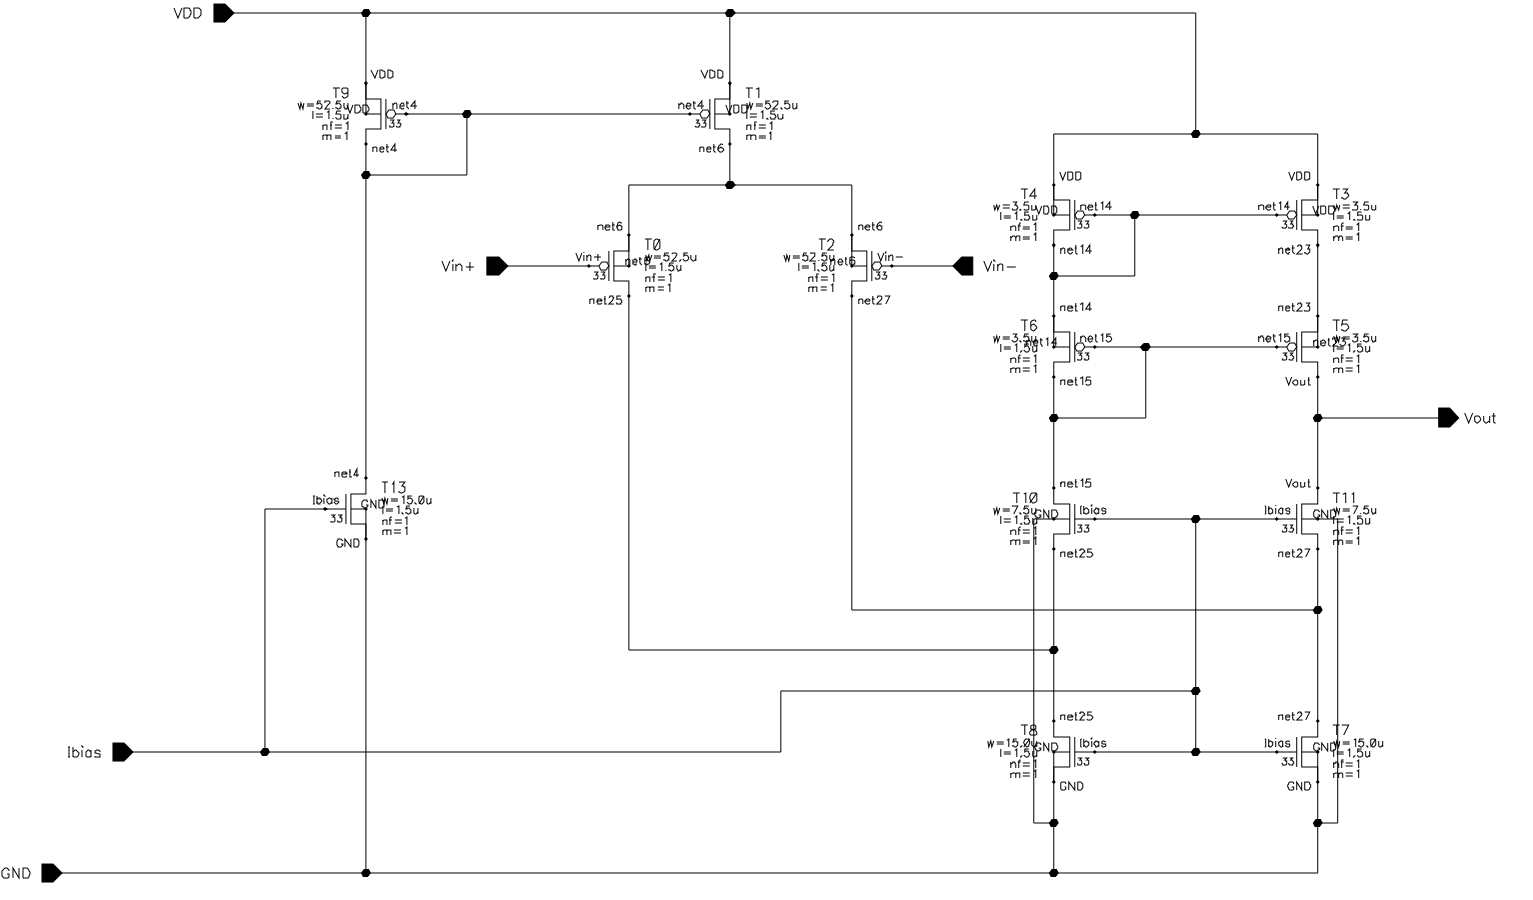
\includegraphics[width=300pt]{OTAsimples.png}\\
  \caption{OTA PMOS simples}\label{OTAsimples}
\end{figure}

\section{Circuito de controle}
O circuito de controle projetado é mostrado na figura \ref{circuitoControle}. Os comparadores utilizados foram implementados como células Gm de alta performance conforme projetadas por \citeonline{azcona-calvo2}. As saídas dos comparadores então conectadas a um latch RS \textit{NAND based}, sendo que o sinal VCH é comparado com um sinal de RESET por um circuito lógico OR (NOR seguido de inversor) antes de chegar à entrada R do latch. Isso é feito para que o estado inicial do latch possa ser setado com um pulso inicial do sinal RESET, impedindo que o circuito inicie com uma condição lógica indefinida.     

\begin{figure}[!ht]
  \centering
  % Requires \usepackage{graphicx}
  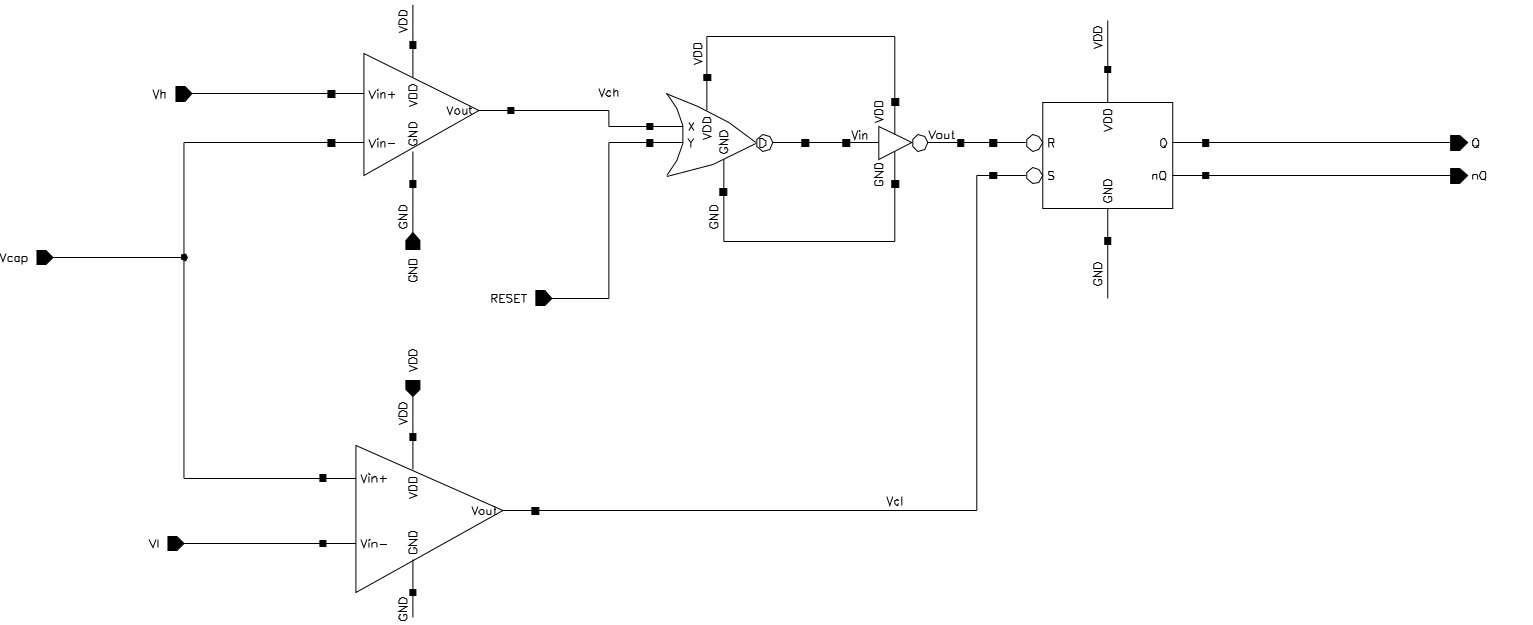
\includegraphics[width=450pt]{circuitoVWC.jpg}\\
  \caption{Circuito de controle}\label{circuitoControle}
\end{figure}

\section{VFC}
O circuito completo do VFC, incluindo dimensionamento dos transistores e valor do capacitor, é mostrado na figura \ref{circuitoVFC}. 1 V e 600 mV foram os valores escolhidos como limites de integração superior e inferior, respectivamente, para o VWC e um capacitor de 25 pF foi utilizado. Estes valores, aliados à faixa de saída das correntes do conversor contribuíram para uma faixa de frequências adequada para o VFC. 

\begin{figure}[!ht]
  \centering
  % Requires \usepackage{graphicx}
  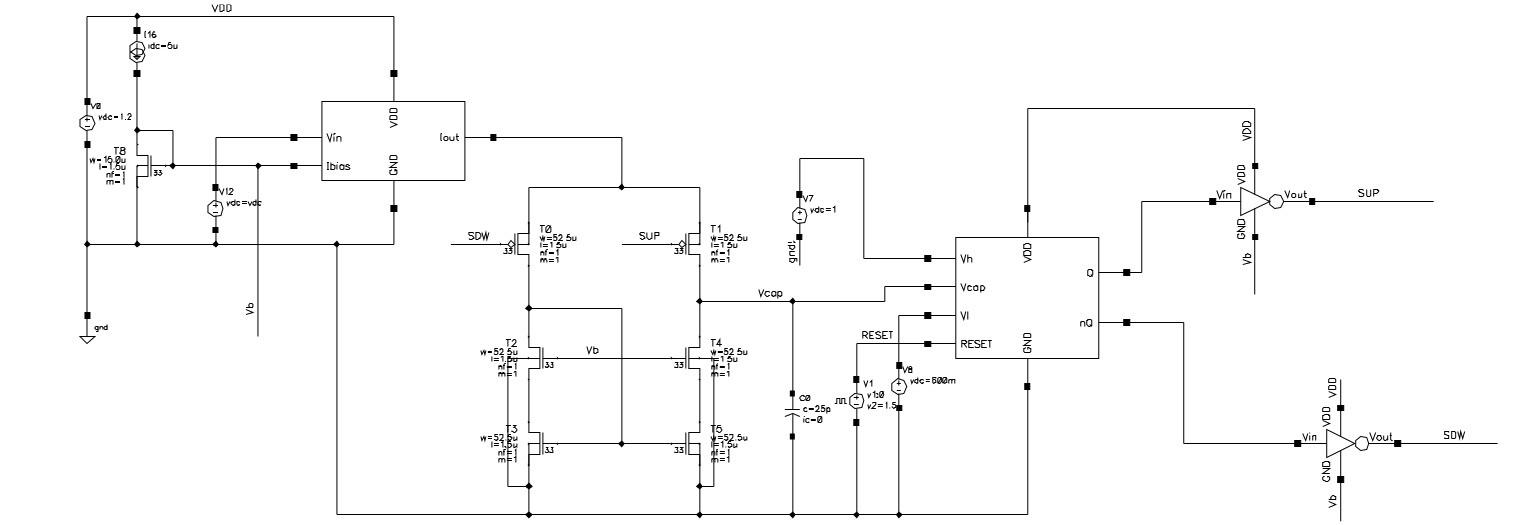
\includegraphics[width=450pt]{circuitoVFC.jpg}\\
  \caption{Circuito VFC}\label{circuitoVFC}
\end{figure}


% ----------------------------------------------------------------
% Experimentos e Resultados *******************
% ----------------------------------------------------------------
\chapter{Experimentos e Resultados}
As simulações a seguir foram realizadas nos circuitos projetados através do uso do simulador Spectre. 

\section{OTA}
\subsection{Resposta DC}
O esquema utilizado para simulação DC do amplificador de transcondutância é mostrado na figura \ref{esquemaOTA_DC}, onde vdc = 1,2 V e idc = 5 $\mu$A. 
\begin{figure}[!ht]
  \centering
  % Requires \usepackage{graphicx}
  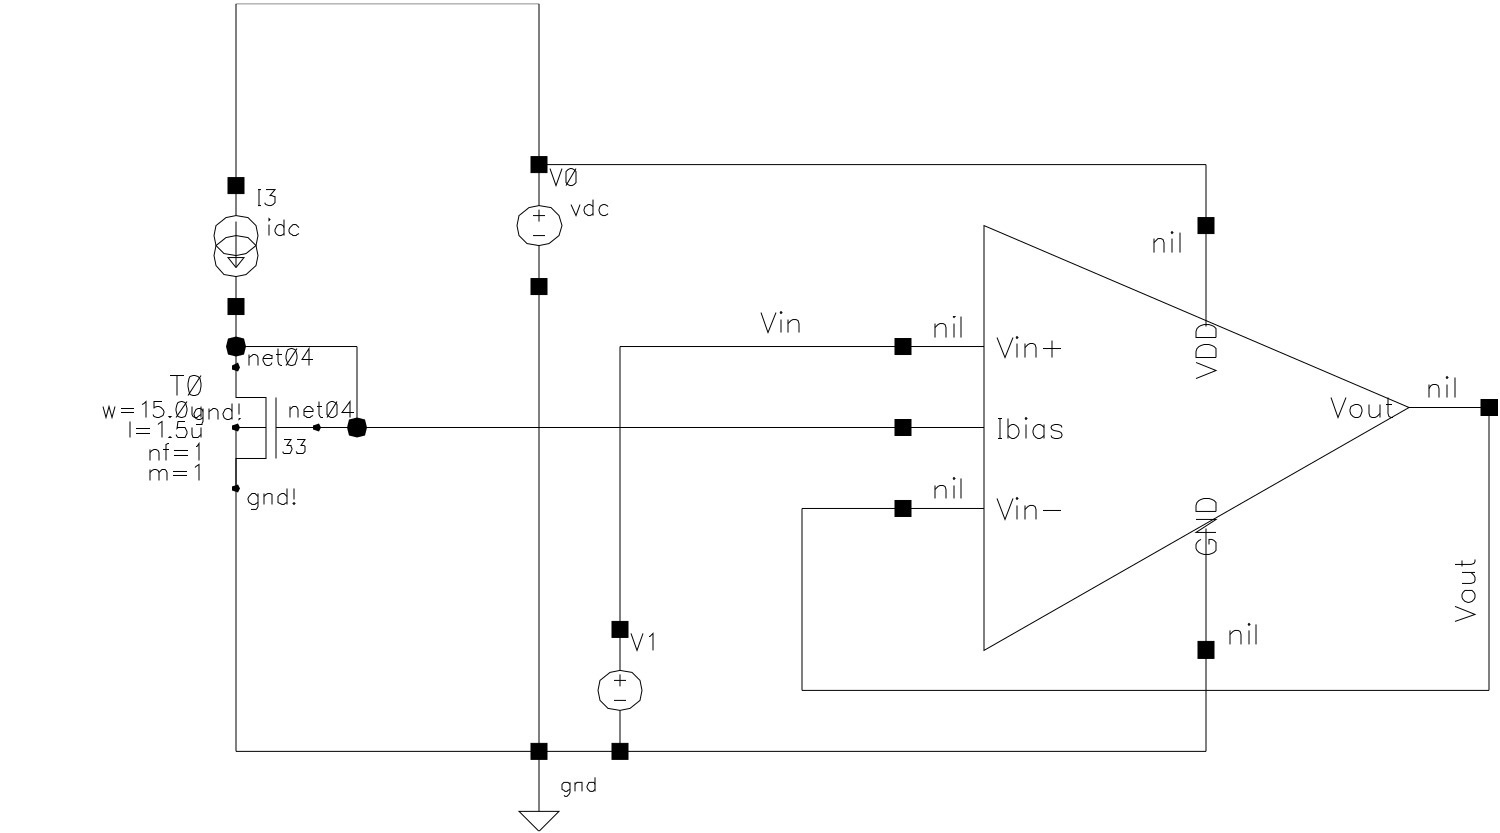
\includegraphics[width=300pt]{esquemaOTA_DC.jpg}\\
  \caption{Esquema para simulação DC}\label{esquemaOTA_DC}
\end{figure}

A figura \ref{resDC} mostra a resposta DC do amplificador de transcondutância \textit{rail-to-rail}. 

\begin{figure}[!ht]
  \centering
  % Requires \usepackage{graphicx}
  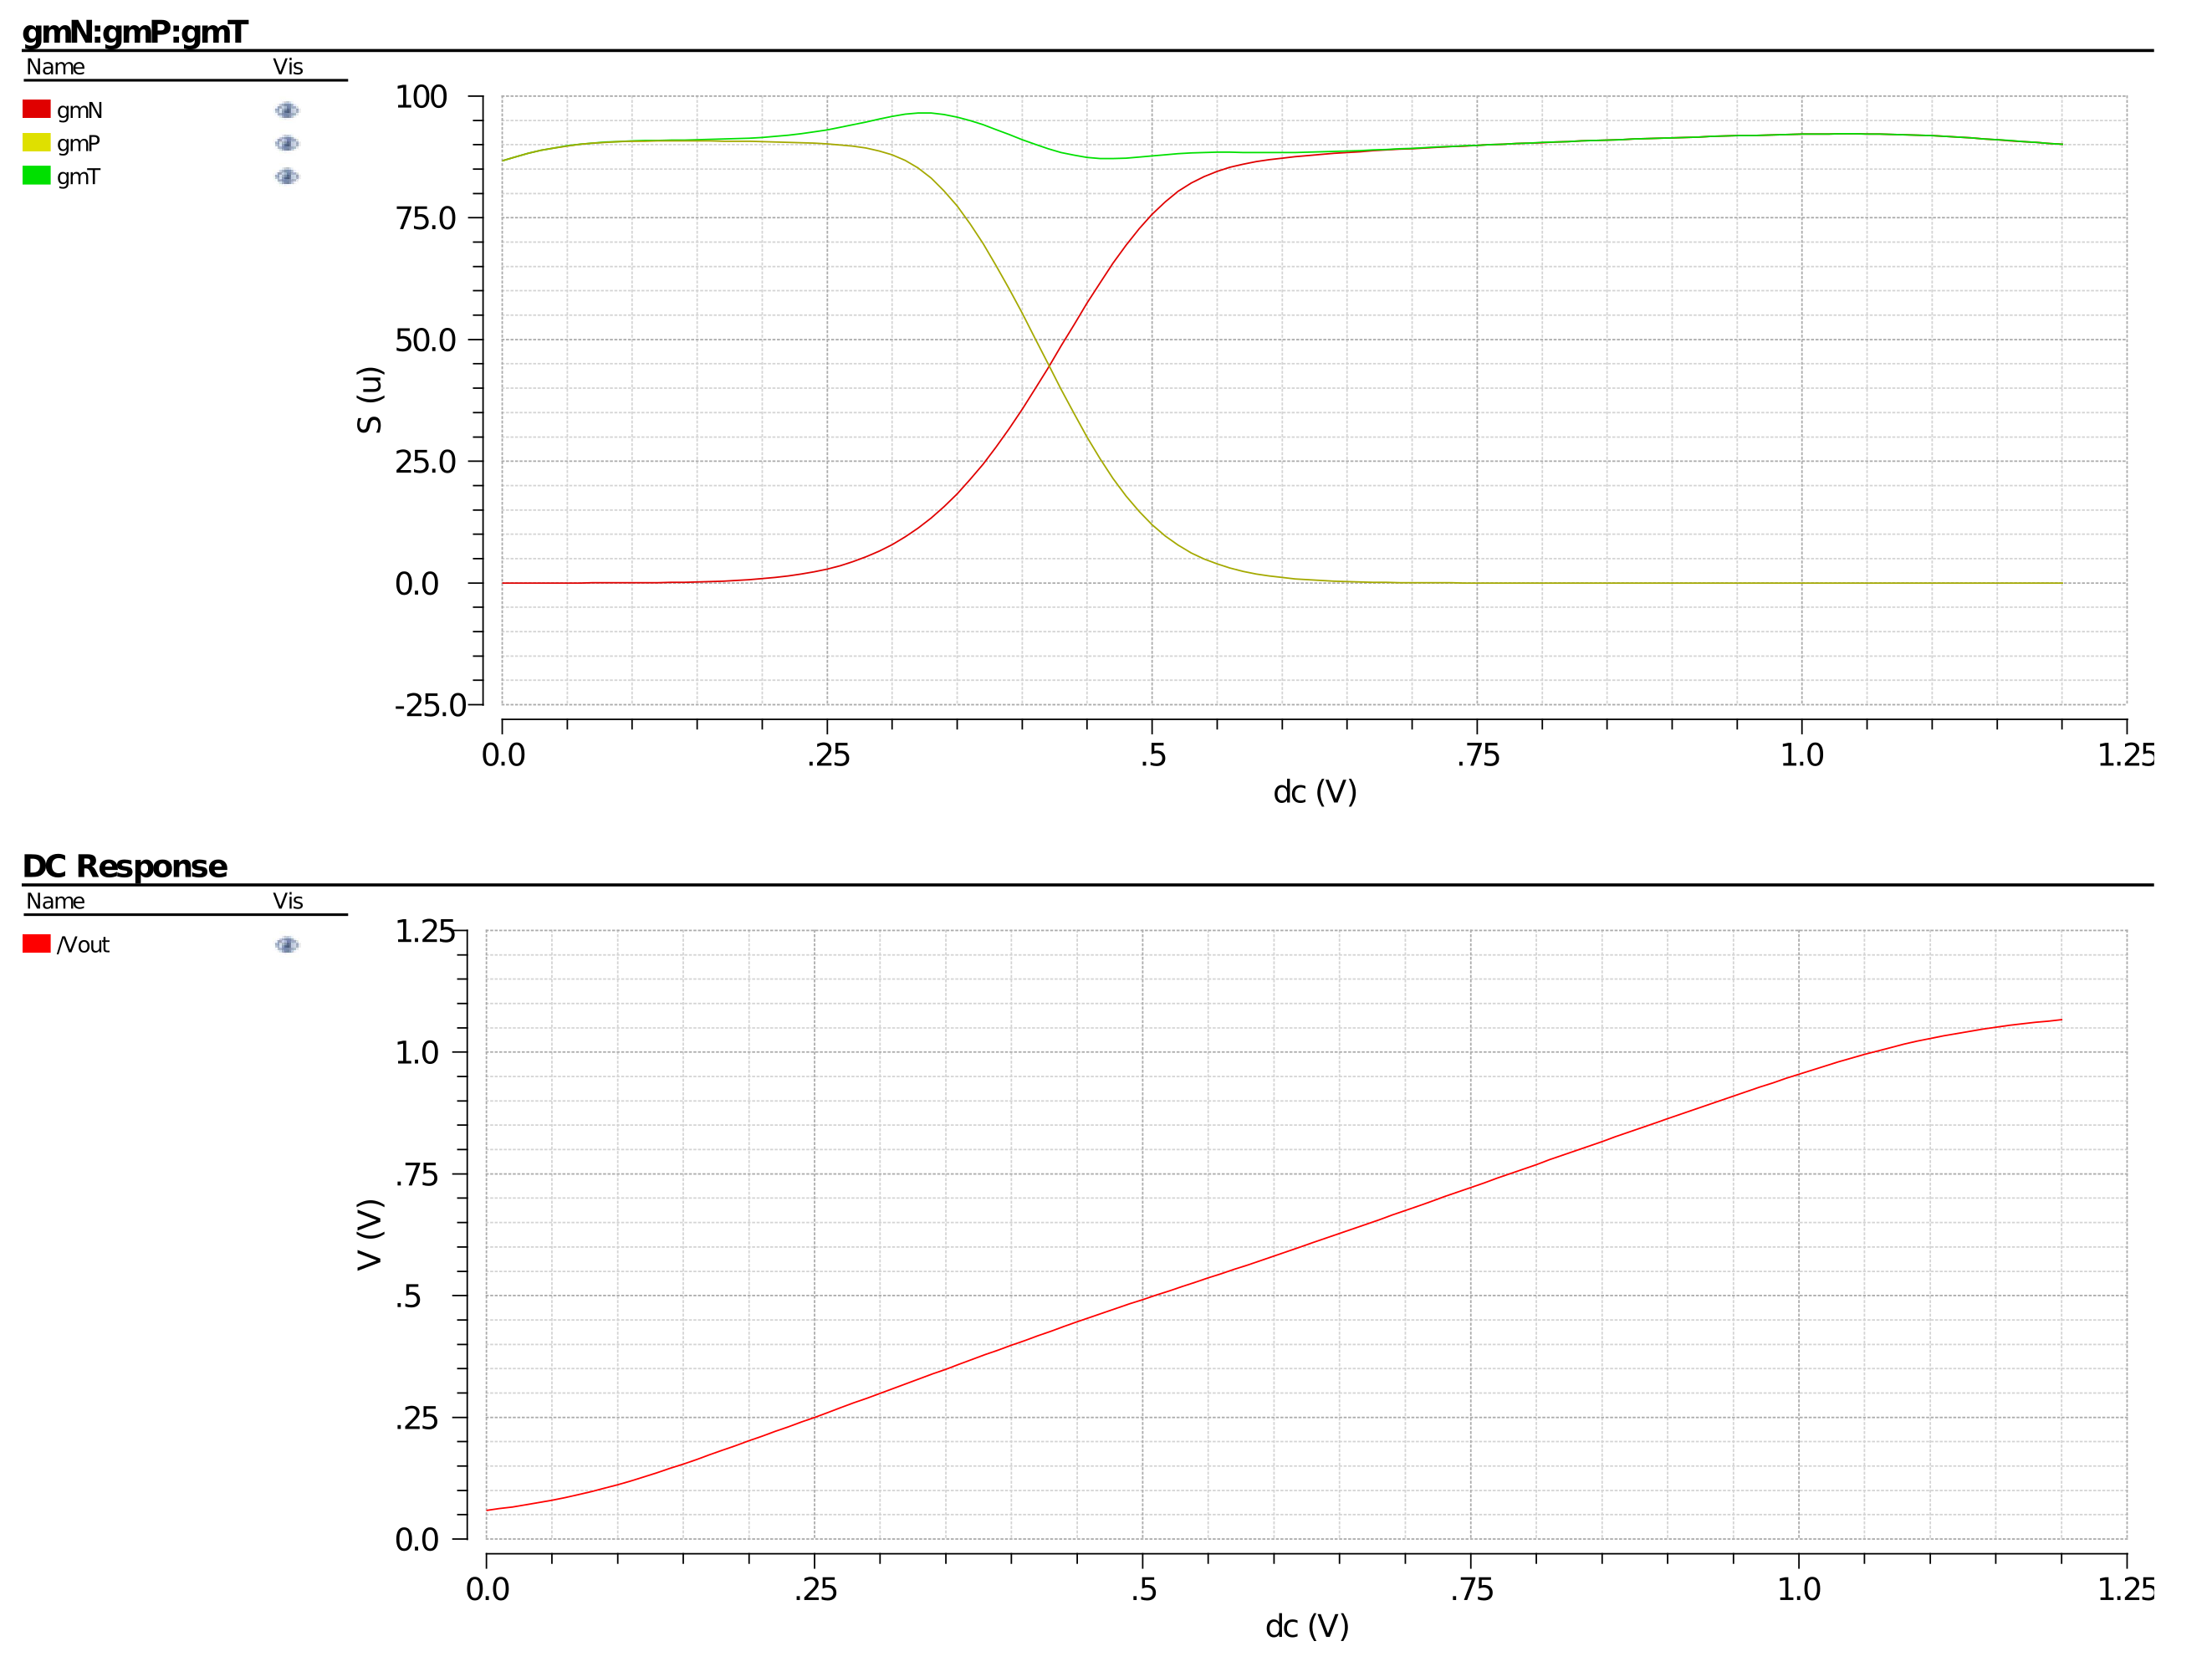
\includegraphics[width=450pt]{OTA_DC.png}\\
  \caption{Simulação DC}\label{resDC}
\end{figure}

O primeiro gráfico apresenta a variação de transcondutância dos pares diferenciais de entrada PMOS e NMOS e também a transcondutância total, sendo essa a soma das transcondutâncias dos pares em paralelo. Observa-se que há transcondutância total por toda a faixa de valores de entrada, confirmando a operação \textit{rail-to-rail} do circuito. Através do uso da técnica de deslocamento de nível, pôde-se obter uma variação máxima na transcondutância total de 5,08\%. 

Já a segunda curva mostra a saída do OTA configurado como \textit{buffer}, conectado em retroalimentação negativa conforme apresentado no esquema da figura \ref{esquemaOTA_DC}, para valores de tensão de entrada variando entre 0 e VDD. A tabela \ref{tabDC} lista todos os resultados. 

\begin{table}[h]
    \begin{center}    
    \begin{tabular}{ | c | c | }
    \hline
    Tensão de alimentação  & 1,2 V \\
    \hline
    Faixa de entrada  & \textit{rail-to-rail} \\ 
    \hline
    Tensão de \textit{offset}  & 59,05 mV \\
    \hline
    Potência  & 23,8 $\mu W $ \\
    \hline
    Variação máxima da transcondutância de entrada  & 5,08 \% \\
    \hline
    \end{tabular}
    \caption[Resultados resposta DC]{Resultados resposta DC}
    \label{tabDC}
    \end{center}
\end{table}

\subsection{Resposta AC}
Na simulação AC, o amplificador apresentou ganho \textit{open loop} de 42,4 dB, largura de banda de 13,8 MHz e slew rate de 27,7 V/$\mu$s. A figura \ref{esquemaOTA_AC} mostra o esquema de simulação montado, e a figura \ref{resAC} e tabela \ref{tabAC} apresentam os resultados obtidos. Novamente, vdc = 1,2 V e idc = 5 $\mu$A.

\begin{figure}[!ht]
  \centering
  % Requires \usepackage{graphicx}
  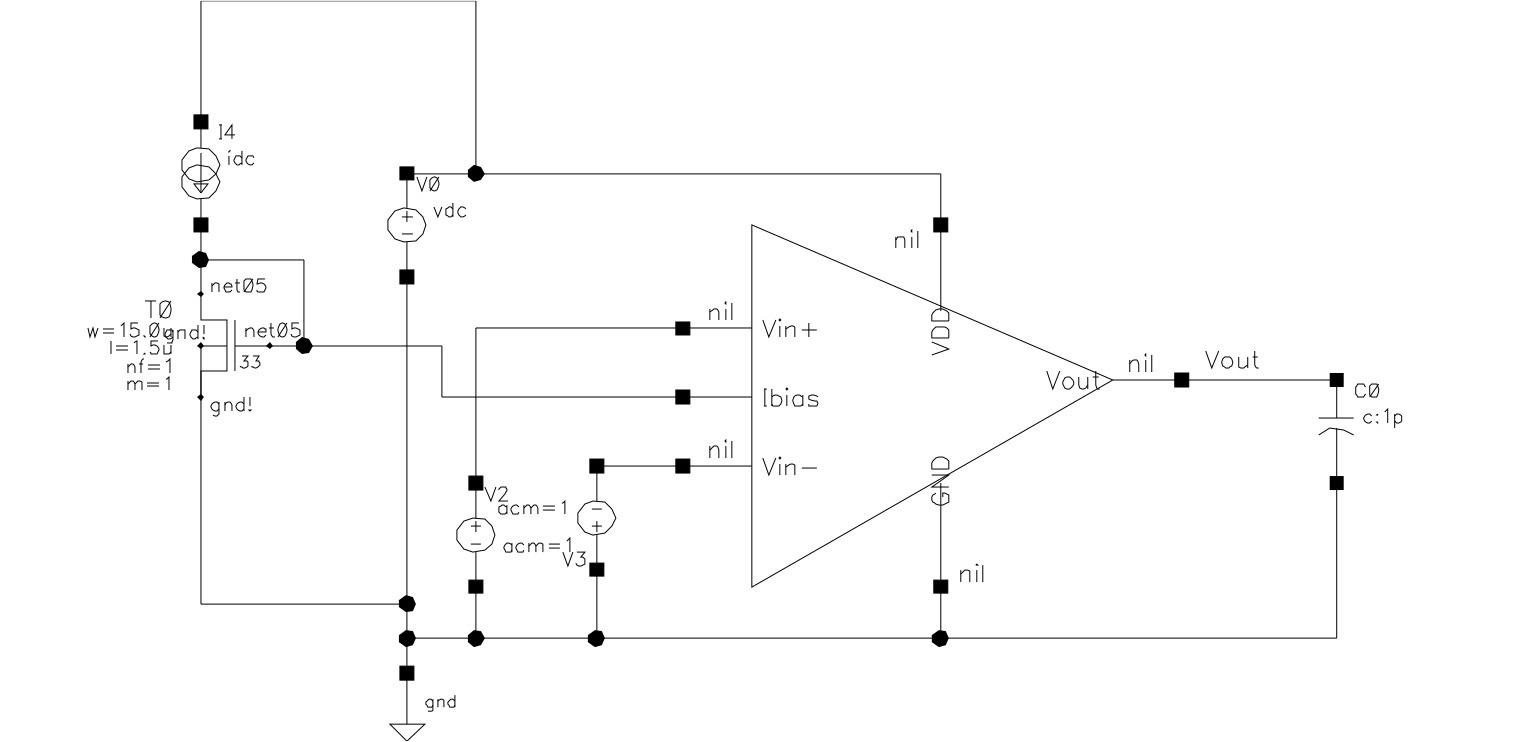
\includegraphics[width=300pt]{esquemaOTA_AC.jpg}\\
  \caption{Esquema para simulação AC}\label{esquemaOTA_AC}
\end{figure}

\begin{figure}[!ht]
  \centering
  % Requires \usepackage{graphicx}
  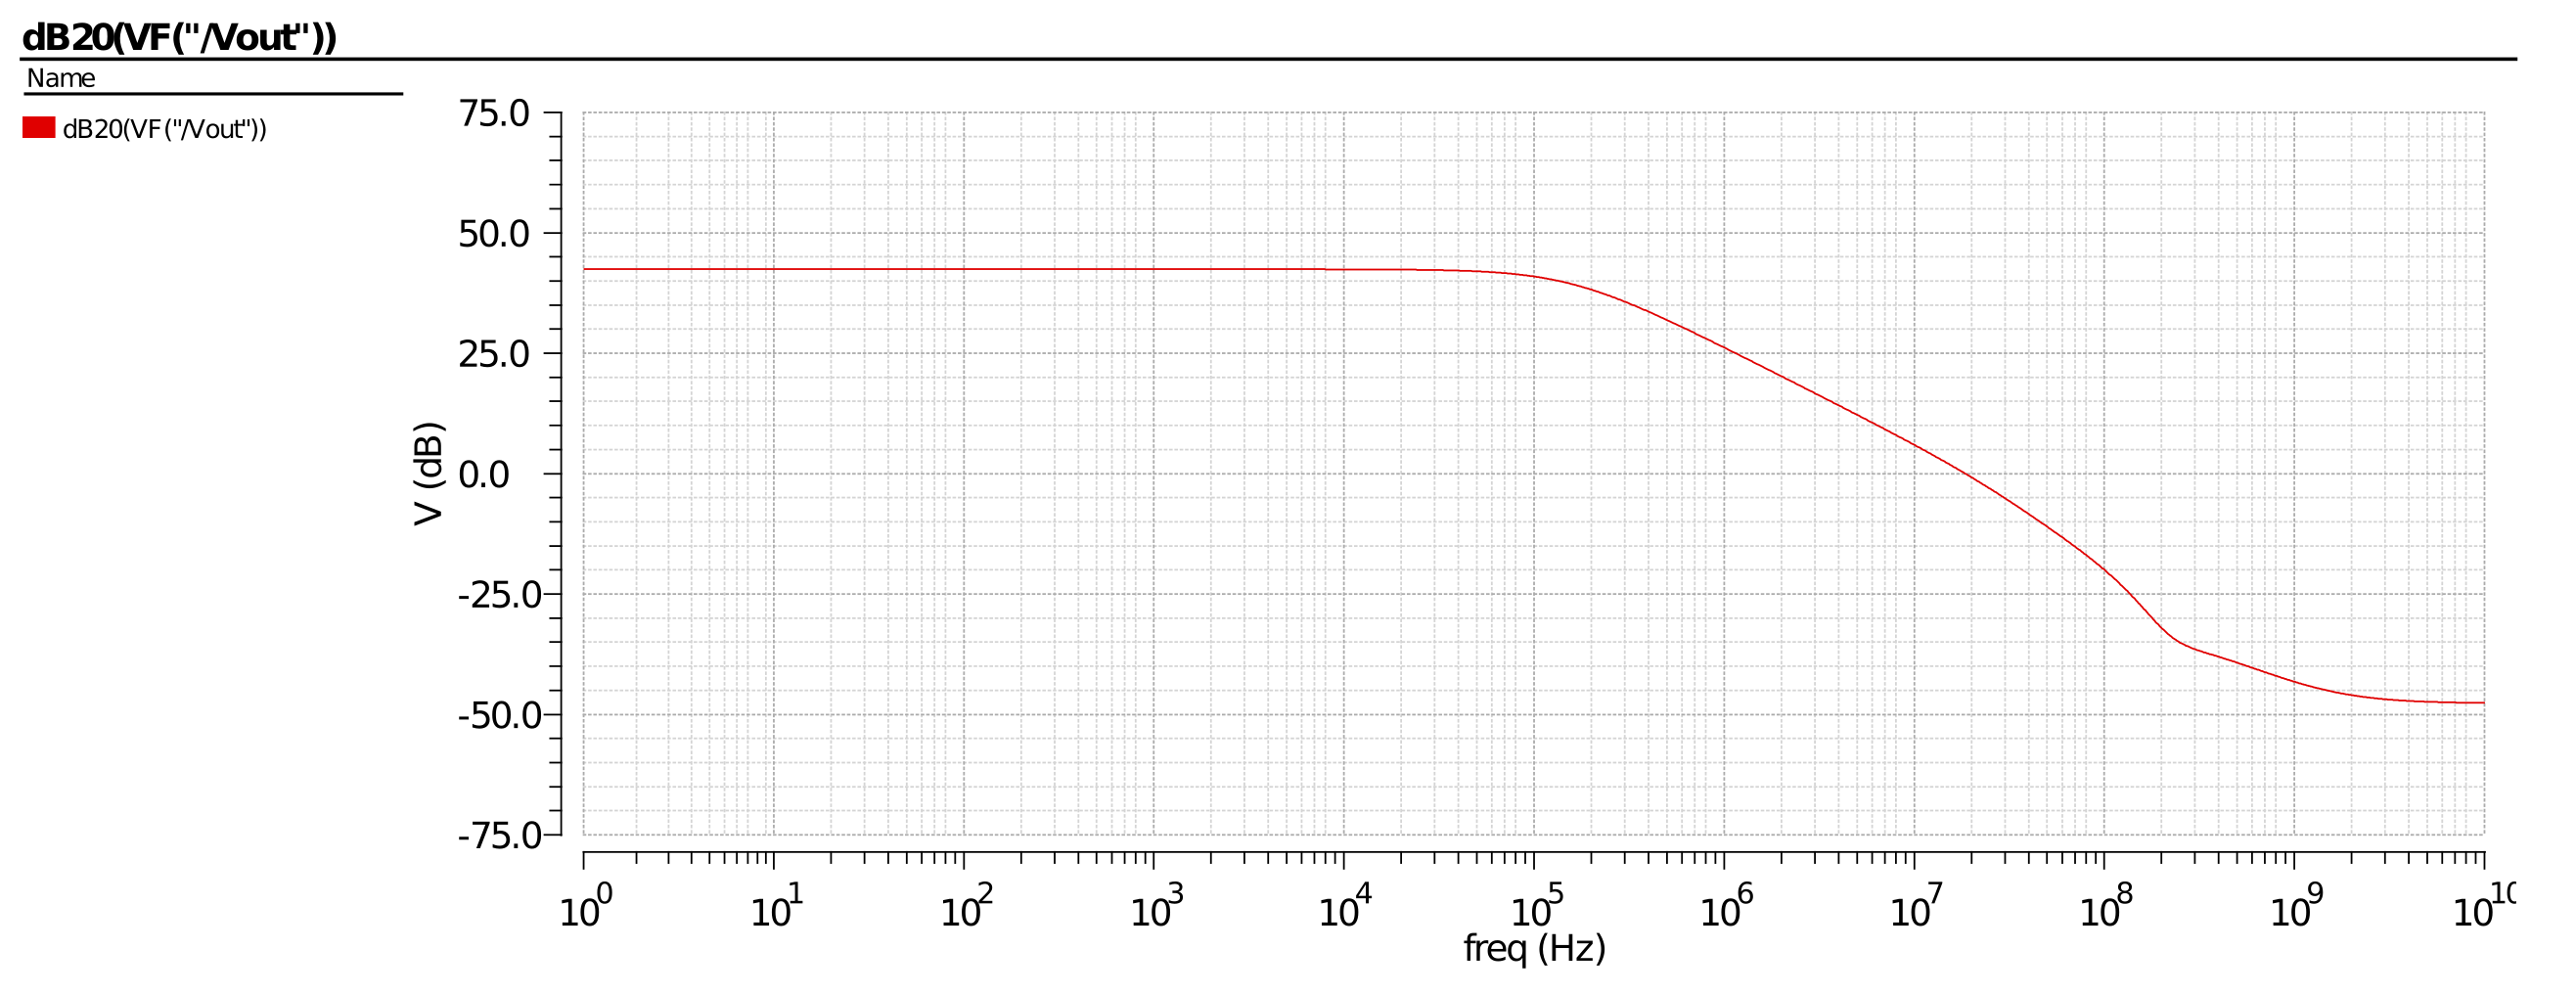
\includegraphics[width=450pt]{OTA_AC.png}\\
  \caption{Simulação AC}\label{resAC}
\end{figure}

\begin{table}[h]
    \begin{center}    
    \begin{tabular}{ | c | c | }
    \hline
    Ganho  & 42,4 dB \\
    \hline
    Margem de ganho  & 13,8 MHz \\ 
    \hline
    Slew Rate  & 27,7 V/$\mu s$ \\
    \hline
    \end{tabular}
    \caption[Resultados resposta AC]{Resultados resposta AC}
    \label{tabAC}
    \end{center}
\end{table}

\clearpage

\section{Conversor V-I}
O conversor V-I apresentou consumo de potência de 98,46 $\mu$W e erro de linearidade de 0,083\%, conforme constam na figura \ref{resFFVA} e tabela \ref{tabFFVA}.

\begin{figure}[!ht]
  \centering
  % Requires \usepackage{graphicx}
  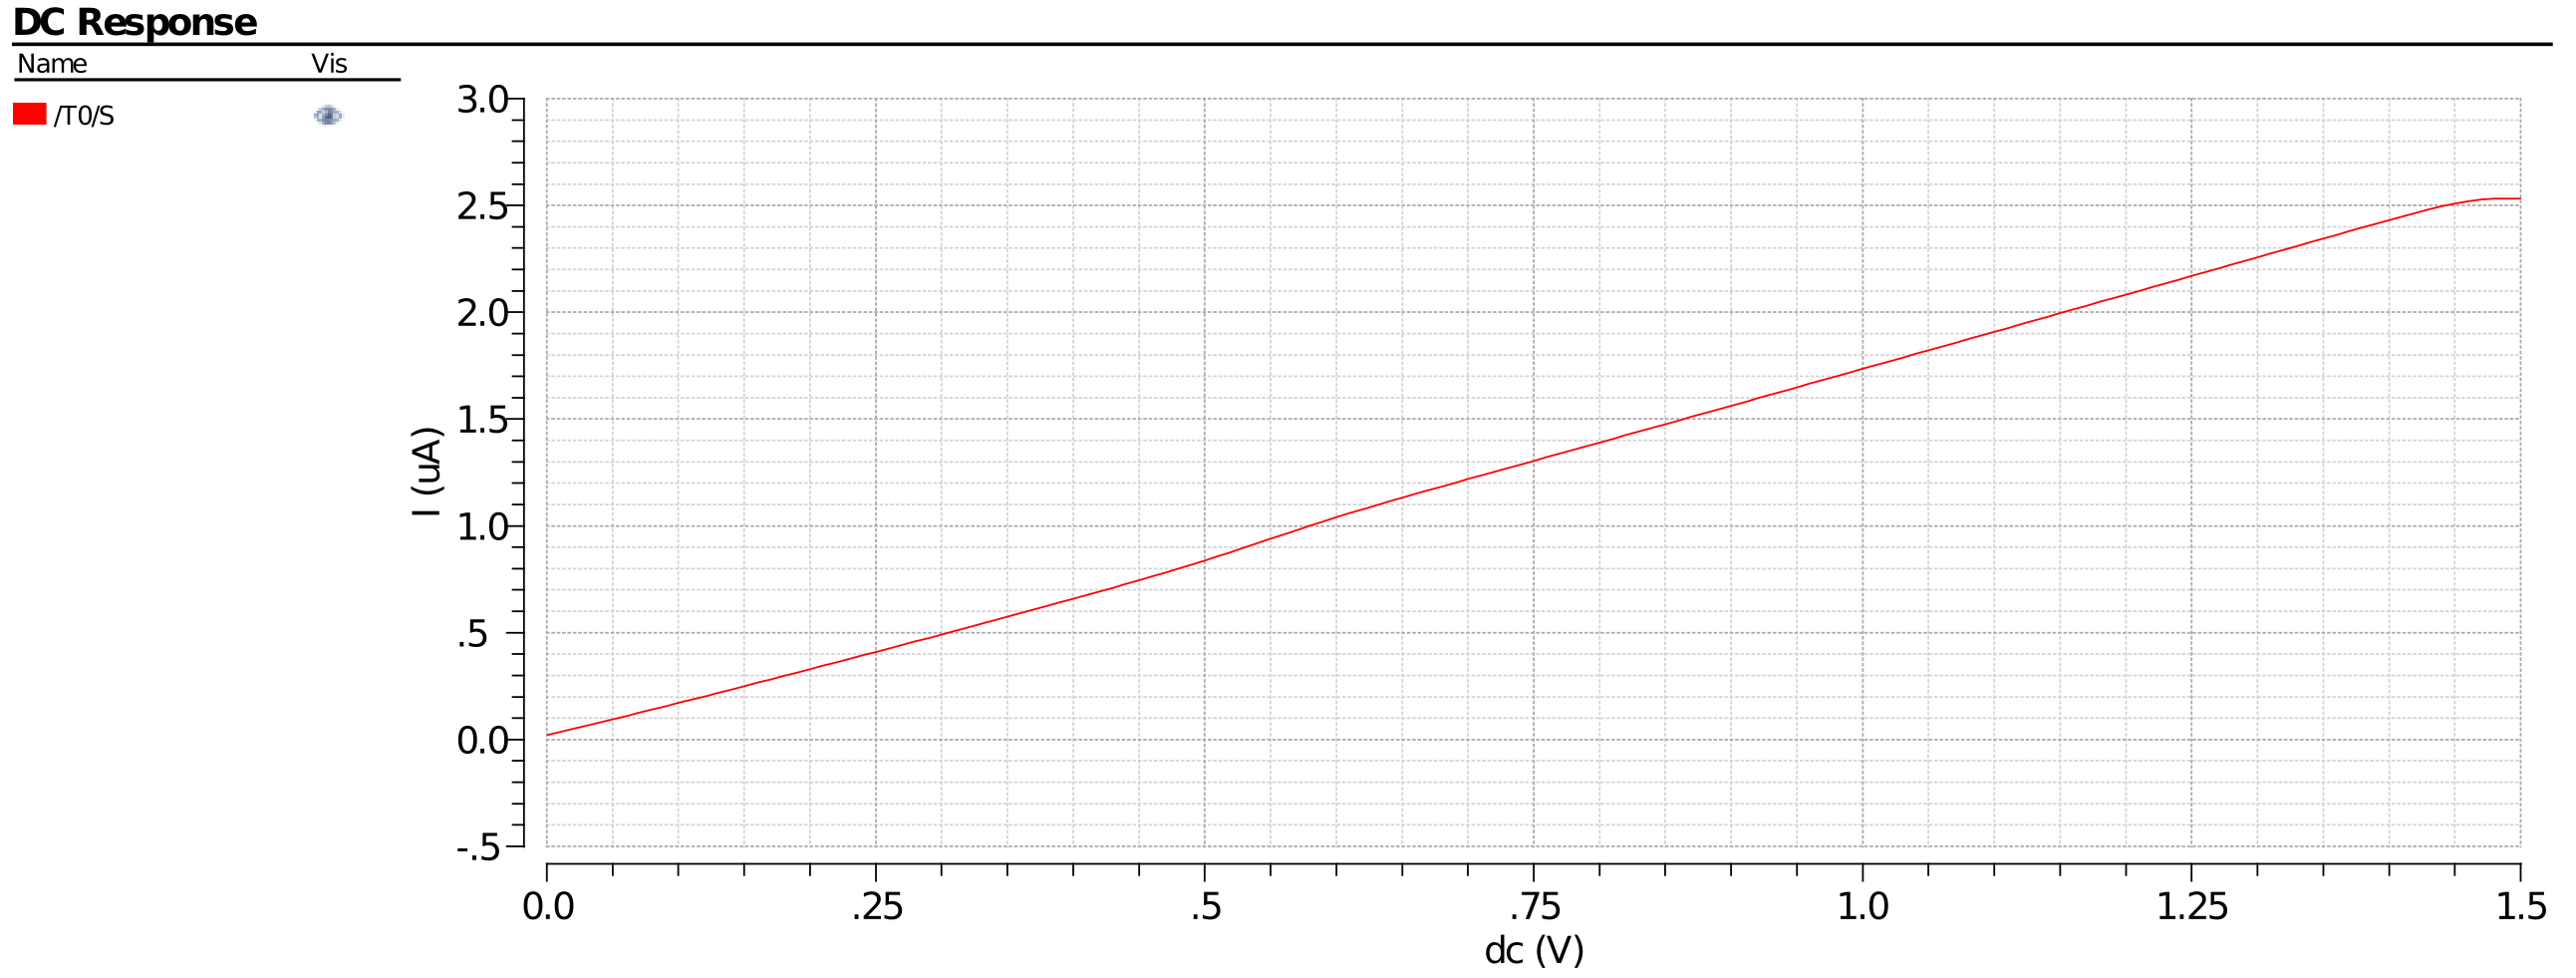
\includegraphics[width=450pt]{resFFVA.png}\\
  \caption{Simulação Conversor V-I}\label{resFFVA}
\end{figure}

\begin{table}[h]
    \begin{center}    
    \begin{tabular}{ | c | c | }
    \hline
    Potência  & 98,46 $\mu W $ \\
    \hline
    Erro de Linearidade  & 0,083 \% \\
    \hline
    \end{tabular}
    \caption[Resultados Conversor V-I]{Resultados Conversor V-I}
    \label{tabFFVA}
    \end{center}
\end{table}

\section{VFC}
Por fim, as respostas obtidas pela simulação do VFC completo são mostradas. O esquema utilizado é o mesmo circuito da figura \ref{VFC_final}.

As figuras \ref{resVFC0}, \ref{resVFC600} e \ref{resVFC12} mostram tanto a saída do circuito quanto a curva de carga do capacitor para tensões de entrada de 0 V, 600 mV e 1.2 V, respectivamente.

\begin{figure}[!ht]
  \centering
  % Requires \usepackage{graphicx}
  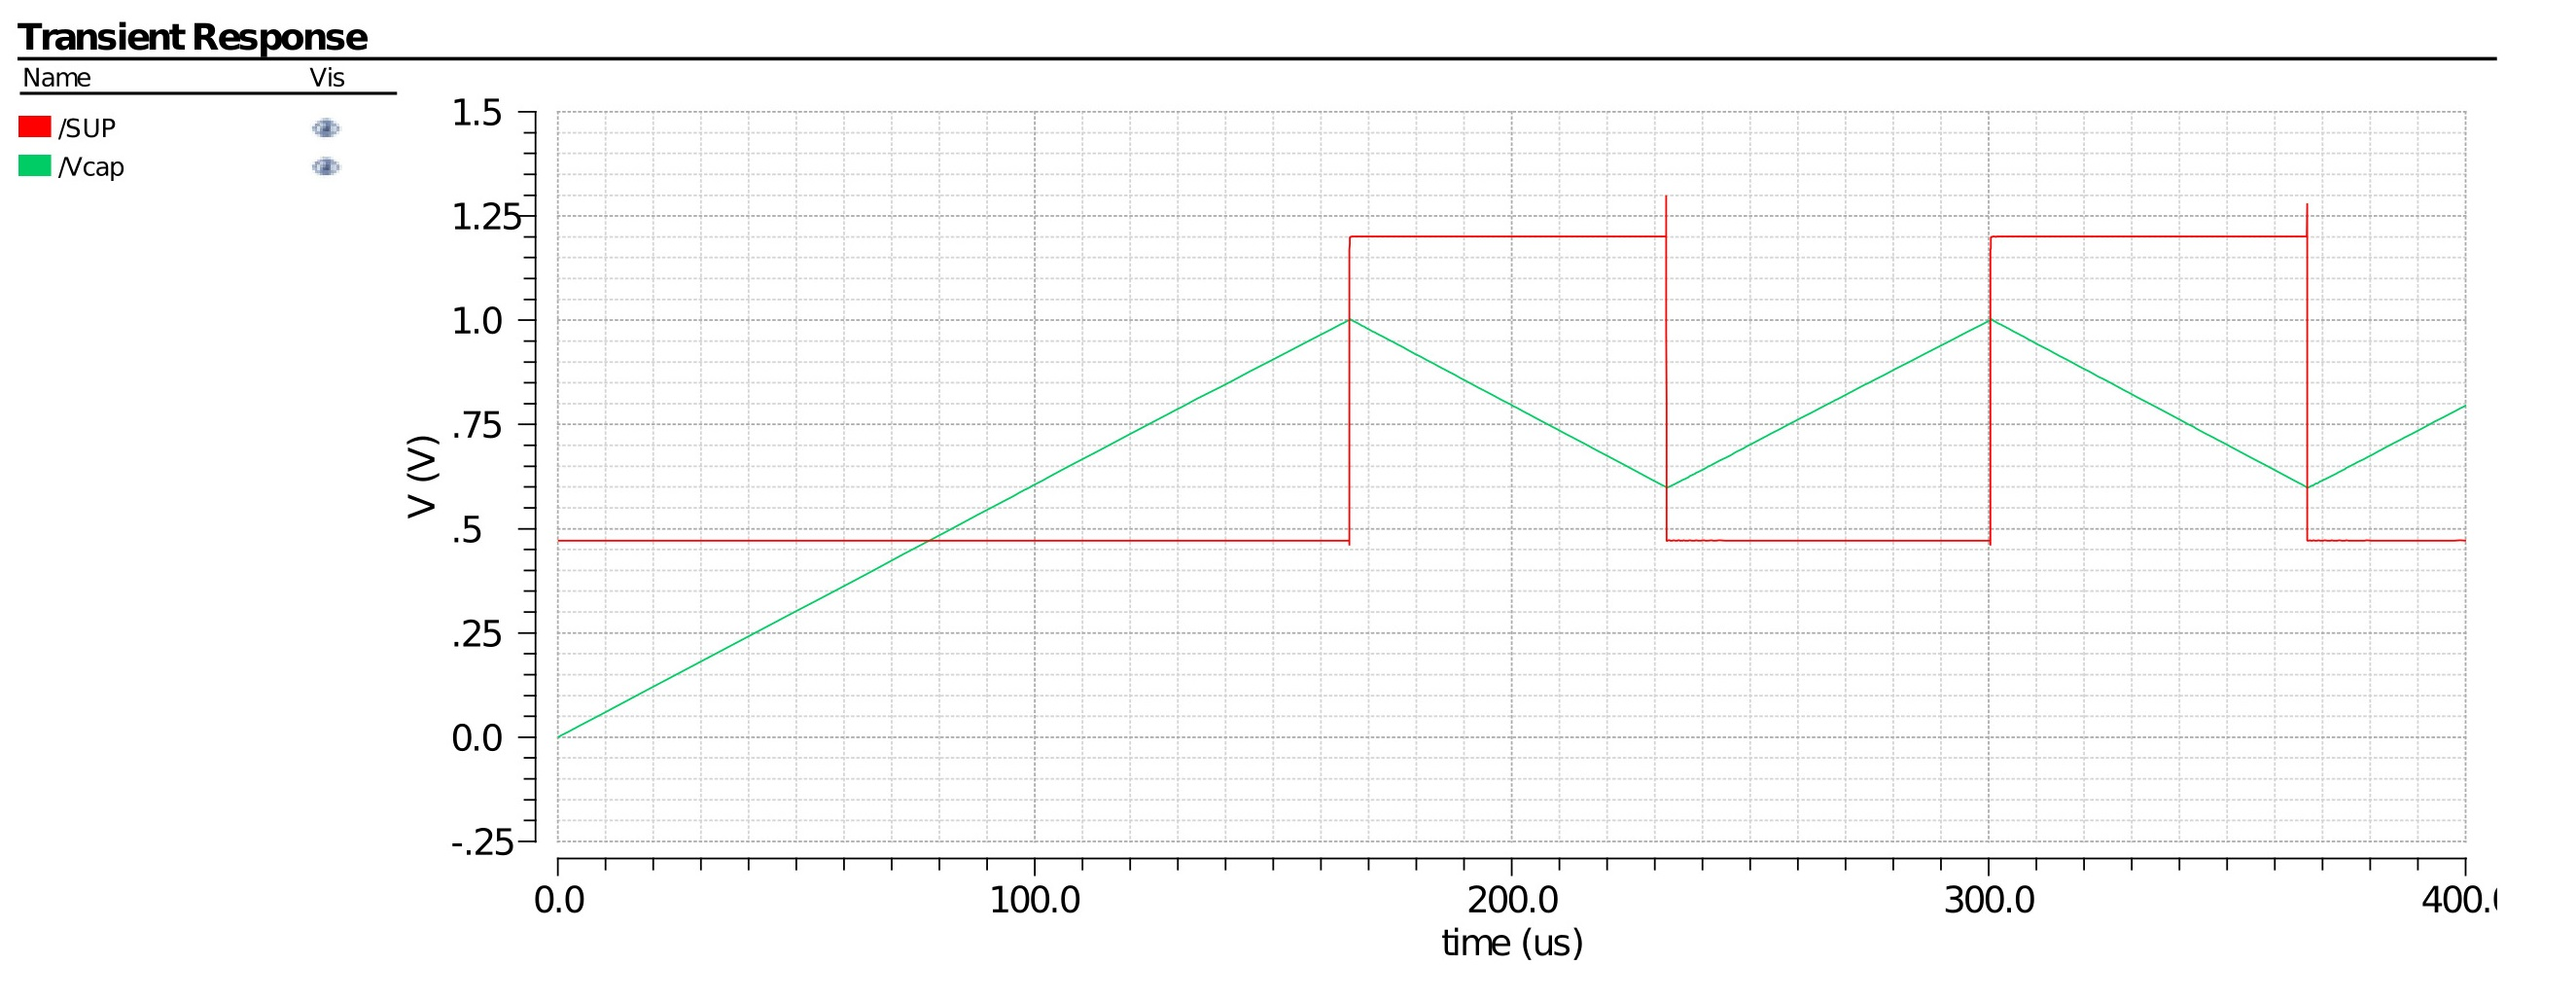
\includegraphics[width=450pt]{saidaVFC0.jpg}\\
  \caption{Simulação transiente VFC para Vin = 0 V}\label{resVFC0}
\end{figure}

\begin{figure}[!ht]
  \centering
  % Requires \usepackage{graphicx}
  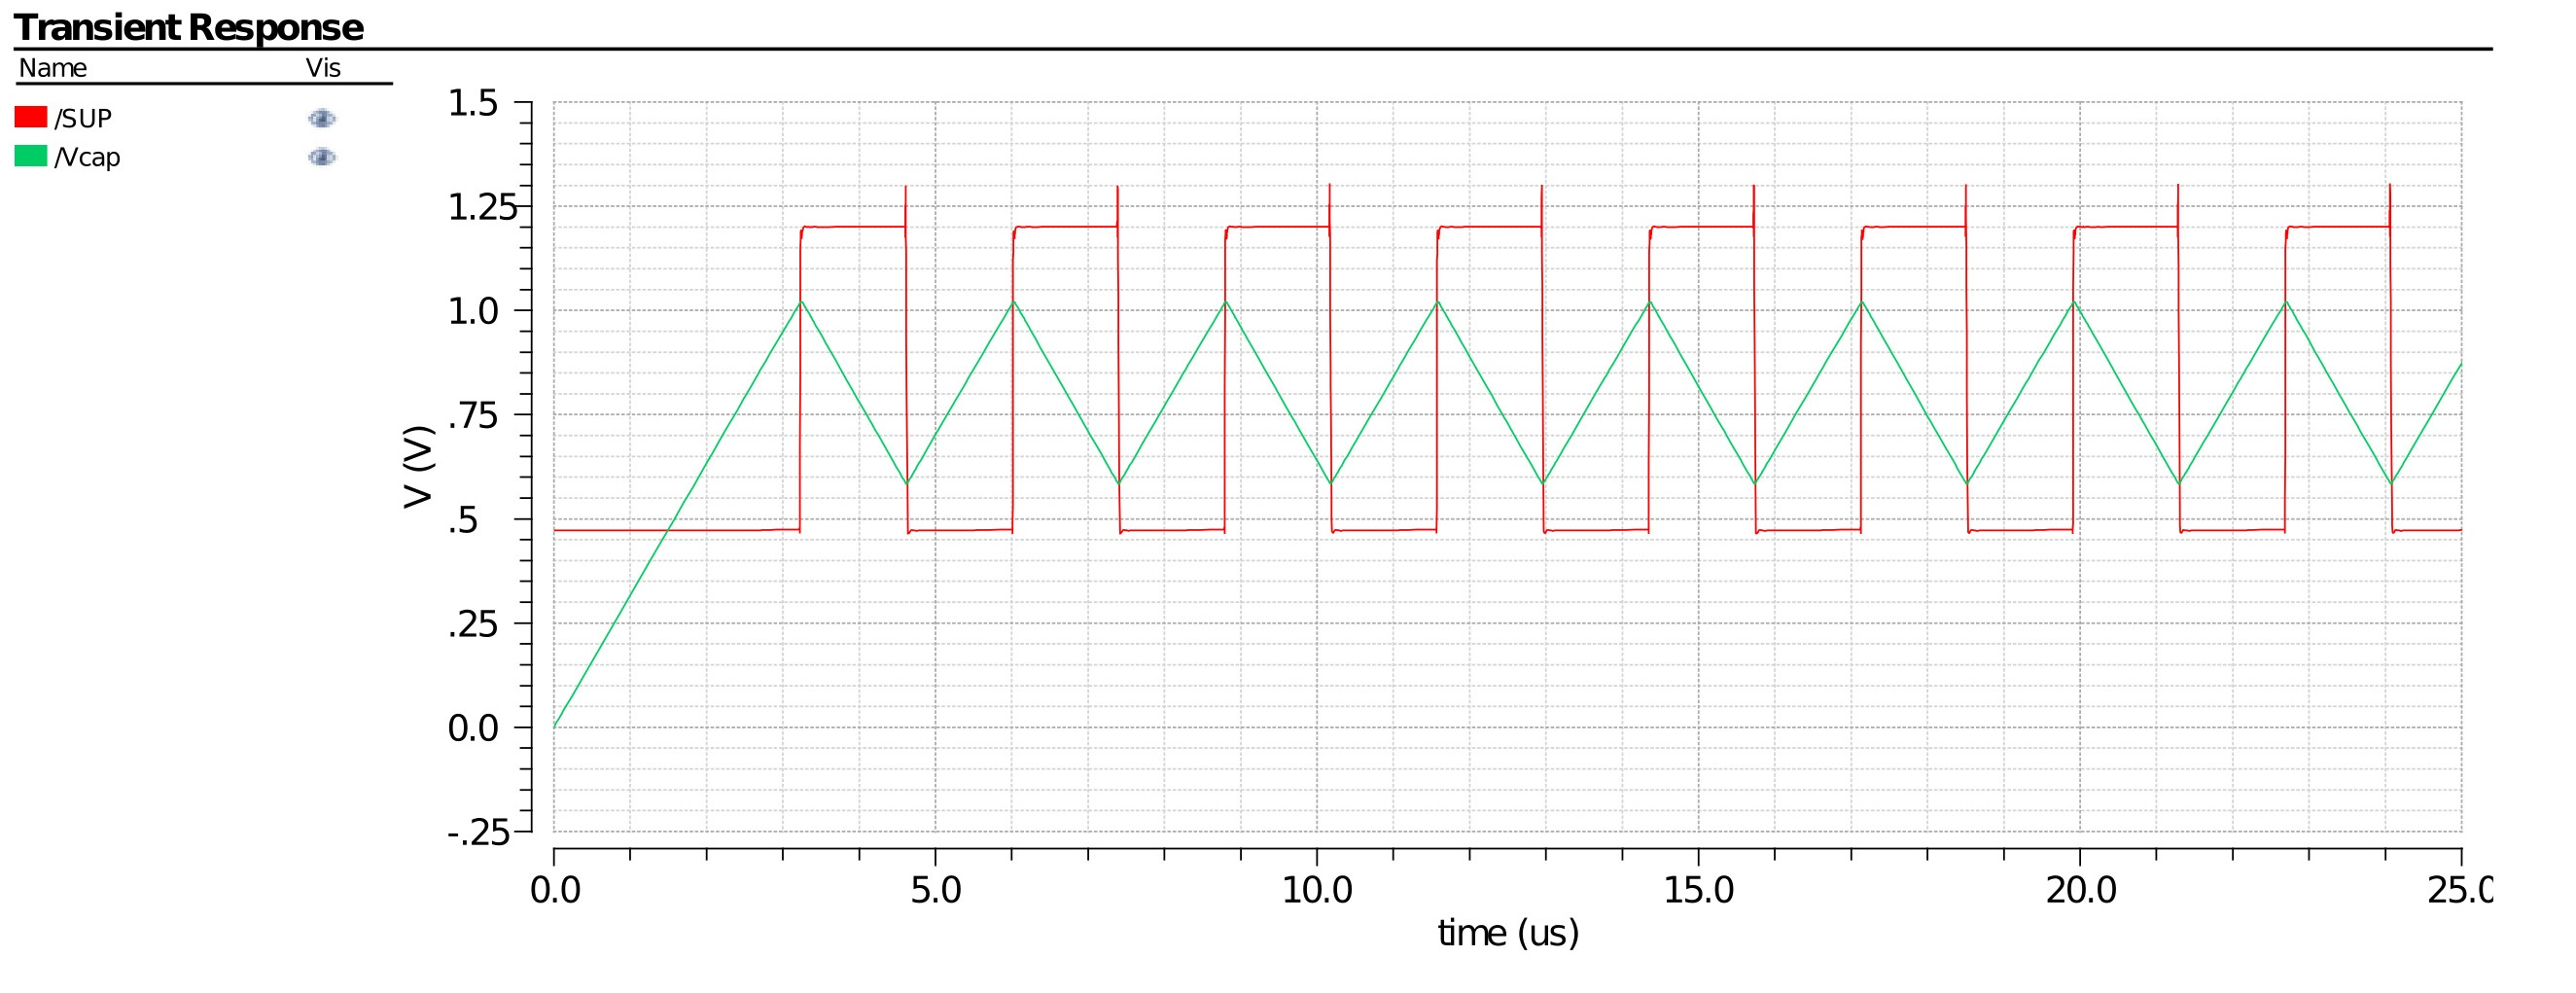
\includegraphics[width=450pt]{saidaVFC600.jpg}\\
  \caption{Simulação transiente VFC para Vin = 600 mV}\label{resVFC600}
\end{figure}

\begin{figure}[!ht]
  \centering
  % Requires \usepackage{graphicx}
  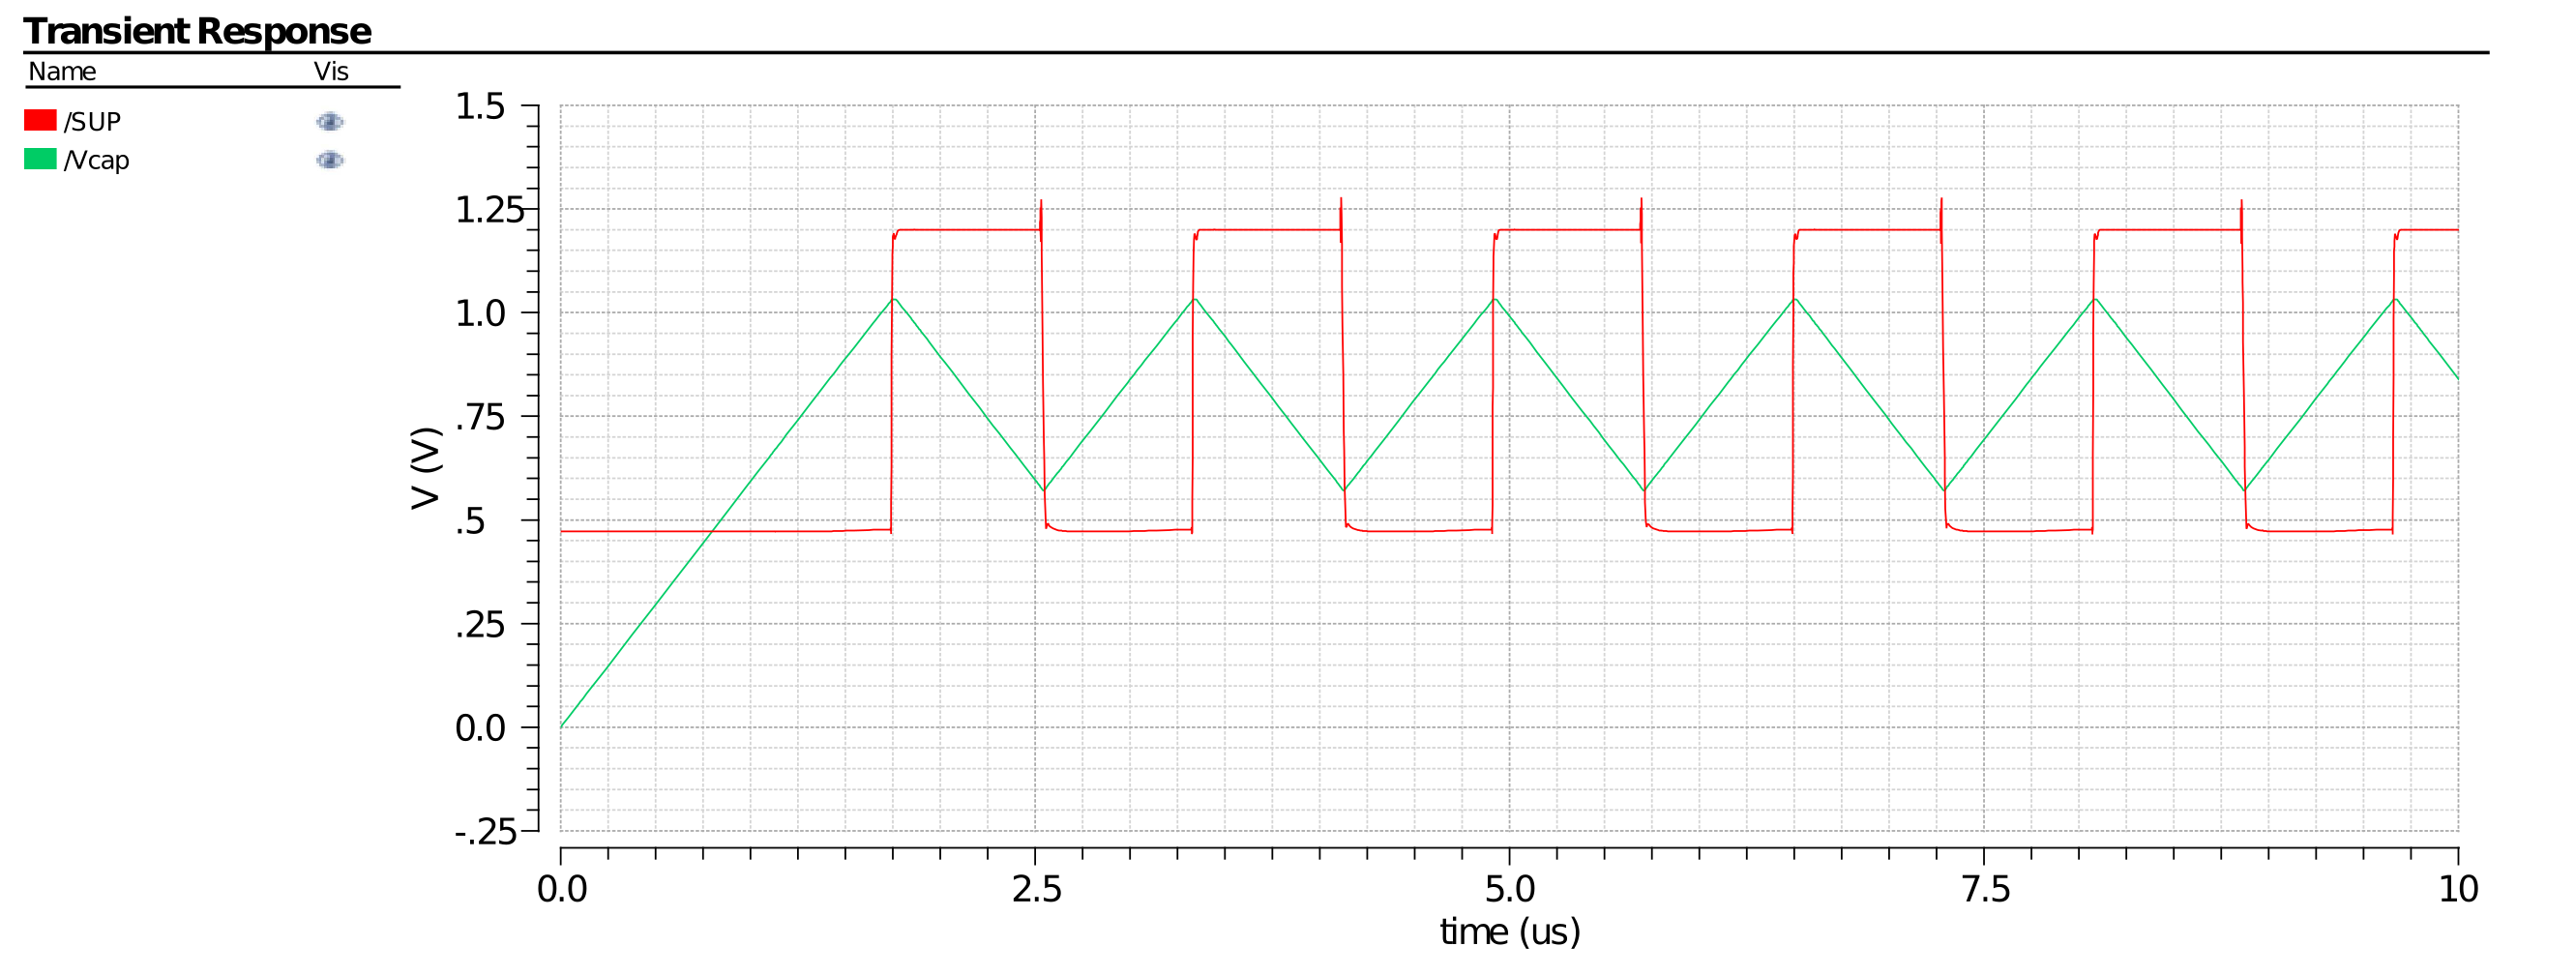
\includegraphics[width=450pt]{saidaVFC12.png}\\
  \caption{Simulação transiente VFC para Vin = 1.2 V}\label{resVFC12}
\end{figure}

A figura \ref{resVFC} foi obtida através de dados gerados por uma simulação paramétrica do circuito, onde a frequência do sinal de saída do VFC foi medida para 15 valores de Vin entre 0 e 1.2V. Esses dados foram plotados com auxílio do software MATLAB, o qual também calculou a regressão linear que gerou a reta em laranja que pode ser observada na figura. Para valores de entrada acima de 1,1 V, observou-se perda considerável de linearidade, portanto a faixa de entrada do circuito foi considerada como sendo de 0 V a 1,1 V.

Dessa forma, houve um erro de linearidade de 0,49\%, definido como \(1-R^2\), onde $R^2$ é o coeficiente de linearidade. O circuito apresentou consumo de potência de 424 $\mu$W

\begin{figure}[!ht]
  \centering
  % Requires \usepackage{graphicx}
  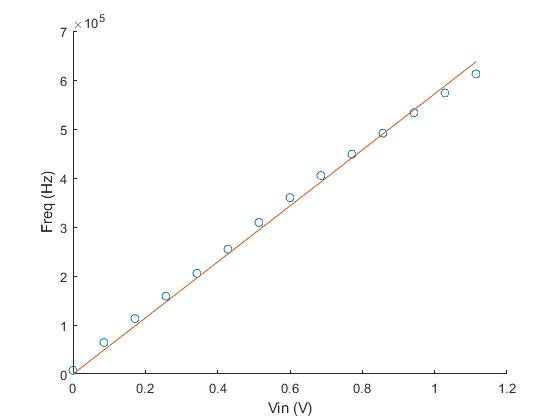
\includegraphics[width=300pt]{saidaVFC.jpg}\\
  \caption{Simulação VFC}\label{resVFC}
\end{figure}

\begin{table}[h]
    \begin{center}    
    \begin{tabular}{ | c | c | }
    \hline
    Potência  & 424 $\mu W $ \\
    \hline
    Faixa de entrada  & 0 V - 1,1 V \\
    \hline
    Faixa de saída  & 7,44 kHz - 606,1 kHz \\
    \hline
    Erro de Linearidade  & 0,49 \% \\
    \hline
    \end{tabular}
    \caption[Resultados VFC]{Resultados VFC}
    \label{tabVFC}
    \end{center}
\end{table}


% ----------------------------------------------------------------
% Conclusão e Trabalhos Futuros *******************
% ----------------------------------------------------------------
\chapter{Conclusão}
Em aplicações de baixo consumo, conversores tensão-frequência são alternativas atrativas a ADCs convencionais por seu baixo custo, simplicidade e imunidade a ruídos. Na última década, a preferência por esses dispositivos em aplicações portáteis, como as WSNs, mostrou-se crescente.

Neste trabalho, foi proposto o projeto de um VFC multivibrador com entrada \textit{rail-to-rail}, tensão de alimentação abaixo de 1,8V, consumo de potência abaixo de 1 mW e resposta razoavelmente linear nas frequências de saída para tensões de entrada. Tal dispositivo foi projetado dadas as motivações anteriores, e foi pensado para uma possível aplicação em redes de sensores sem fio.

Após breve revisão bibliográfica sobre o assunto, foi feito o projeto dos três blocos que compõem o conversor. Para estes, foi escolhido como bloco de entrada dois OTAS, sendo um com entrada \textit{rail-to-rail} e outro implementado com um par diferencial PMOS simples, em configuração FFVA. Para o bloco integrador, utilizou-se um capacitor aliado a um circuito de carga e descarga de baixo consumo. Por fim, o bloco de controle foi projetado através da implementação de um VWC construído com comparadores de célula Gm e um latch SR. 

Os circuitos projetados foram simulados utilizando-se simulador Spectre e os resultados analisados com a resposta do simulador e o software MATLAB. Da análise dos dados observou-se bons resultados tanto para o OTA \textit{rail-to-rail} projetado, com este apresentando variação máxima na transcondutância de entrada de 5,08\%, consumo de 23,8 $\mu W$ e margem de ganho de 13,8 MHz, quanto para o Conversor V-I implementado com ele, o qual consumiu 98,46 $\mu W$ e apresentou alta linearidade, com um erro de 0,083\%. Já o circuito final do VFC apresentou consumo de potência razoável de 424 $\mu W$ e erro de linearidade de 0,49\%. Apesar de alto em comparação com outros trabalhos similares observados na literatura, esse valor ainda é aceitável dado o escopo do projeto. A faixa de saída de 7,44 kHz a 606,1 kHz está de acordo com o valor máximo de 2Mhz especificado e a extensão do sinal de entrada mostrou-se quase \textit{rail-to-rail}. 

Dados estes resultados, fica como proposta para trabalhos futuros a otimização dos circuitos lógicos dos dispositivos digitais, como latches e portas lógicas (que estão além do escopo deste projeto) a fim de reduzir o erro de linearidade. Também para este propósito, outra medida não inclusa neste trabalho mas que pode ser considerada em trabalhos futuros é a realização de simulações FFT para caracterizar a distorção harmônica do OTA e, com os dados obtidos, otimizar o circuito para melhor servir à aplicação. Compensação contra variações de temperatura é também algo desejável que pode ser explorado futuramente.      


% ----------------------------------------------------------
% ELEMENTOS PÓS-TEXTUAIS
% ----------------------------------------------------------
\postextual
% ----------------------------------------------------------

% ----------------------------------------------------------
% Referências bibliográficas
% ----------------------------------------------------------
\bibliography{TFGdanilo33248}

% ----------------------------------------------------------
% Glossário
% ----------------------------------------------------------
%
% Consulte o manual da classe abntex2 para orientações sobre o glossário.
%
%\glossary

% ----------------------------------------------------------
% Apêndices
% ----------------------------------------------------------

% ---
% Inicia os apêndices
% ---
% \begin{apendicesenv}

% % Imprime uma página indicando o início dos apêndices
% \partapendices
% % ----------------------------------------------------------
% \chapter{Quisque libero justo}
% % ----------------------------------------------------------
% \lipsum[50]

% \end{apendicesenv}
% ---



\end{document}
